

\chapter{集合与映射}

这一章我们首先介绍了集合的定义、集合的运算、集合的关系, 然后利用集合的关系定义了映射, 并利用映射研究了集合的可数性. 这些内容是全书的基础.

\section{集 合}

\section*{1. 集合的定义}

集合这个名词是由德国数学家G·Can tor在1874年首先提出的. 这是一个至今没有严格数学定义 的概念. 为了完备起见, 我们直接采用Cantor原话作为我们的定义.

定义 “集合是由我们直观感觉或意识 到的、确 定的、不同对象汇集而成的一个整体. 这些对象称为此集合的元素(成员)”或点.

通常用大写字母 $A\text{ 、 }B\text{ 、 }X\text{ 、 }Y\text{ 、 }\Omega \cdots \cdots$ 表示集合,而用小写字母 $a\text{ 、 }b\text{ 、 }x\text{ 、 }y\text{ 、 }\omega \cdots \cdots$ 表示集合的元素.

若 $a$ 是集合 $A$ 的元素,则称 $a$ 属于 $A$ ,记为 $a \in  A$ ,若 $a$ 不是集合 $A$ 的元素,则称 $a$ 不属于 $A$ ,并记为 $a \in  A$ .

只含一个元素 $a$ 的集合称为单点集,记为 $\{ a\}$ ,没有元素的集合称为空集,记为 $\varnothing$ .

表示集合的方法一般是:

1)列举集合的元素 (如果可能的话);

2) 设 $P$ 是一性质, $x$ 是一对象, $P\left( x\right)$ 表示 $x$ 具有性质 $P$ . 由所有具有性质 $P$ 的对象组成的集合记为 $\{ x \mid  P\left( x\right) \}$ .

\section*{例1}

1) 自然数集 $\{ 1,2,3,\cdots \cdots \}$ 记为 $\mathbf{N}$ ,

2) 整数集 $\{ 0, \pm  1, \pm  2,\cdots \cdots \}$ 记为 $\mathbf{Z}$ .

3) 有理数集 $\left\{  {\left. \frac{m}{n}\right| \;m,n \in  \mathbf{Z},n \neq  0,m\text{ 与 }n\text{ 互质 }}\right\}$ 记为 $\mathbf{Q}$ .

4) 实数集记为 $\mathbf{R}$ (它的表示方法将在下一章介绍).

5) 一元二次方程 ${x}^{2} + x - 2 = 0$ 的解的集合记为
$$\left\{  {x \in  \mathbf{R} \mid  {x}^{2} + x - 2 = 0}\right\}  .$$

\section*{2. 集合之间的关系}
$$\therefore y : {x}^{2} + x - 2 = 0,x \in  R\}$$

定义 设 $A\text{ 、 }B$ 是两个集合.

1)若 $x \in  A$ ,则 $x \in  B$ ,则我们称 $A$ 是 $B$ 的子集,或称 $A$ 包含于 $B$ 中,或称 $B$ 包含 $A$ ,记为
$$A \subset  B\text{ 或 }B \supset  A\text{ ; }$$

2) 若 $A \subset  B,B \subset  A$ ,则我们称 $A$ 与 $B$ 相等,记为
$$A = B;$$

3) 若 $A \subset  B,A \neq  B$ ,则我们称 $A$ 是 $B$ 的真子集,或称 $A$ 严格包含于 $B$ 中,或称 $B$ 严格包含 $A$ ,记为
$$A \subsetneq  B\text{ 。 }B \supsetneq  A$$

注意 存在互不包含的集合 $A$ 与 $B$ .

例2 1) 对任一集合 $A,\varnothing  \subset  A$ ;

2) $N \subsetneq  Z \subsetneq  Q \subsetneq  R$ ;

3) $\left\{  {x \in  \mathbf{R} \mid  {x}^{2} + 1 = 0}\right\}   = \varnothing$ ;

4) $\left\{  {x \in  \mathbf{R} \mid  {x}^{2} + x - 2 = 0}\right\}   = \{ 1, - 2\}$ ;

5) 集合 $\{ {2k} \mid  k \in  \mathbf{N}\}$ 与 $\{ {2k} + 1 \mid  k \in  \mathbf{N}\}$ 互不包含.

\section*{3. 集合的运算及性质}

定义 设 $A\text{ 、 }B$ 是两个集合.

1) $A$ 与 $B$ 的并集,记为 $A \cup  B$ ,定义为
$$A \cup  B\overset{ \bigtriangleup  }{ = }\overset{\left( 1\right) }{ = }\{ x \mid  x \in  A\text{ 或 }x \in  B\} ;$$

2) $A$ 与 $B$ 的交集,记为 $A \cap  B$ ,定义为
$$A \cap  B = \{ x \mid  x \in  A\text{ 并且 }x \in  B\} ;$$

3) $B$ 关于 $A$ 的差集,记为 $A - B$ ,定义为
$$A - B \triangleq  \{ x \mid  x \in  A\text{ 但 }x \in  B\} ;$$

4) 若 $B \subset  A$ ,则称 $A - B$ 为 $B$ 在 $A$ 中的余集或补集,记为 ${C}_{A}B$ . 如果在上、下文中 $A$ 与 $B$ 的关系很清楚,则可简记 ${C}_{A}B$ 为 ${B}^{c}$ .

\begin{center}
	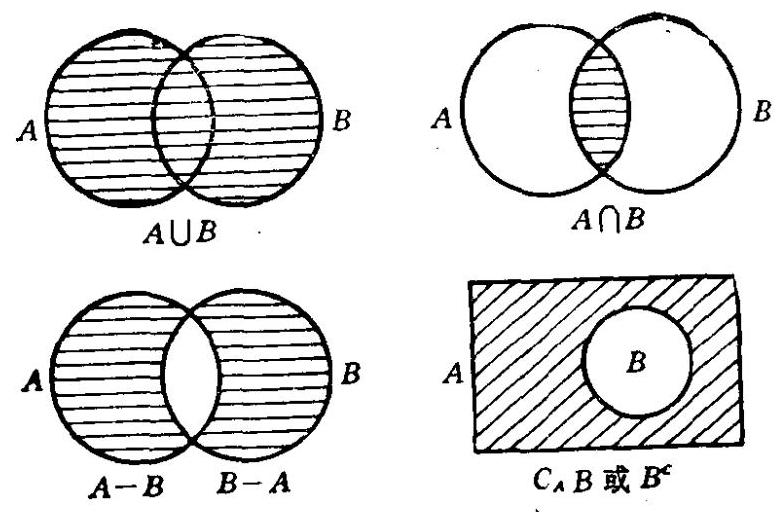
\includegraphics[max width=0.6\textwidth]{images/bo_d25ksc77aajc738obdgg_15_458_918_780_512_0.jpg}
\end{center}
\hspace*{3em} 

图 1-1

例 3 记 $\mathrm{I}$ 为无理数集,则
\begin{align*}
	&Q \cup  I = R,Q \cap  I = \varnothing ,Q = R - I,I = R - Q,\\
	&\mathbf{I} = {C}_{\mathrm{R}}\mathbf{Q} = {\mathbf{Q}}^{c},\;\mathbf{Q} = {C}_{\mathrm{R}}\mathbf{I} = {\mathbf{I}}^{c}.
\end{align*}

定理 $1 \cdot  1 \cdot  1$ 设 $E\text{ 、 }F\text{ 、 }G$ 是三个集合,则

1)并、交都是可交换的,即 $E \cup  F = F \cup  E,\;E \cap  F = F \cap  E;$ 

2) 并、交都是可结合的, 即 $E \cup  \left( {F \cup  G}\right)  = \left( {E \cup  F}\right)  \cup  G,E \cap  \left( {F \cap  G}\right)  = \left( {E \cap  F}\right)  \cap  G$ 


3) 并关于交是可分配的, 即 $x \in  E \cup  F$ 所以 $x \in  F$ 且 $x \in  G$  $x \in  E \cap  \left( {F \cup  G}\right)$ 3 如图9所示,交关于并是可分配的,即

\footnote{
	
	① $\triangleq$ 为规定、约定符号,以下同.
	
}

DeMprgan 公式:$E - \left( {F \cap  G}\right)  = \left( {E - F}\right)  \cup  \left( {E - G}\right)$ 

证明类似.$\therefore {x}^{2} = {52}$ 公式公式设 $x \in  E - \left( {F \cap  G}\right)$ ,则 解: $h$  $\therefore 2 : 3,3 : 4$  $x \in  E,x \in  F \cap  G \Rightarrow  \text{ ① }x \in  E;x \in  F$ 或 $x \in  G$  $\Rightarrow  x \in  E - F$ 或 $x \in  E - G$

$\Rightarrow  x \in  \left( {E - F}\right)  \cup  \left( {E - G}\right) .\checkmark$

因此 $E - \left( {F \cap  G}\right)  \subset  \left( {E - F}\right)  \cup  \left( {E - G}\right)$ .

再证 $\left( {E - F}\right)  \cup  \left( {E - G}\right)  \subset  E - \left( {F \cap  G}\right)$ .

设 $x \in  \left( {E - F}\right)  \cup  \left( {E - G}\right)$ ,则

$x \in  E - F$ 或 $x \in  E - G \Rightarrow  x \in  E,x \in  F$ 或 $x \in  E,x \in  G$

$\Rightarrow  x \in  E;x \notin  F \cup  G$

$\Rightarrow  x \in  E - \left( {F \cap  G}\right)$ .

因此 $\left( {E - F}\right)  \cup  \left( {E - G}\right)  \subset  E - \left( {F \cap  G}\right)$ .

综合上述所证, $E - \left( {F \cap  G}\right)  = \left( {E - F}\right)  \cup  \left( {E - G}\right)$ .

附注 若 $F \subset  E,G \subset  E$ ,则De Morgan 公式的第二式可直接从第一式推得.

\footnote{
	
	① $\rightarrow$ 逻辑符号, $P \rightarrow  Q$ 表示命题 $P$ 推出命题 $Q,P \Leftrightarrow  Q$ 表示 $P\text{ 、 }Q$ 两命题等价
	
}

(2) $x \in  E \subseteq  E$ 总是 $x$ 表 $F$ 消除 $x \in  E$ 正 $F$ 正整数

事实上,分别用 $E - F$ 与 $E - G$ 代换第一式中的 $F$ 与 $G$ 得
$$E - \left( {\left( {E - F}\right)  \cap  \left( {E - G}\right) }\right)  = \left( {E - \left( {E - F}\right) }\right)  \cup  \left( {E - \left( {E - G}\right) }\right)
= F \cup  G\text{ . }$$

由于 $\left( {E - F}\right)  \cap  \left( {E - G}\right)  \subset  E$ ,故
$$E - \left( {F \cup  G}\right)  = \left( {E - F}\right)  \cap  \left( {E - G}\right) .$$

任意多个集合的并与交

定义 以集合作为元素的集合称为集族或集系.

通常用花体字母 $\mathcal{A}$ 或 $\mathcal{B}$ 等来表示集族或集系.

例 4 设 $X$ 是任一集合,由 $X$ 的所有子集组成的集族称为 $X$ 的幂集,记为 ${2}^{X}$ .

例5 设 $\Lambda$ 是一非空集合. 对 $\Lambda$ 的每一元素 $\lambda$ ,规定集合 $X$ 的一子集 ${X}_{\lambda }$ ,由这些子集组成的集族记为 ${\left\{  {X}_{\lambda }\right\}  }_{\lambda  \in  \Lambda }$ ,并称之为依 $\Lambda$ 赋予指标的集族。集合 $\Lambda$ 称为此集族的指标集, $\Lambda$ 的元素称为指标. $\left\{  {{a}_{1}{a}_{2}\cdots {a}_{n}}\right\}$ 很少不是

比如平面上以点 ${M}_{0}$ 为中心以 $n \in  \mathbf{N}$ 为半径的圆盘
$$\bar{B}\left( {{M}_{0},n}\right)  = \left\{  {M \mid  \overline{{M}_{0}M} \leq  n}\right\}$$

的全体构成一个以 $\mathrm{N}$ 为指标集的集族 ${\left\{  \bar{B}\left( {M}_{0},n\right) \right\}  }_{n \in  \mathrm{N}}$ .

定义 设 $\omega$ 是任一非空集族。1)

1) $\mathcal{A}$ 中的元素的并,记为 $\mathop{\bigcap }\limits_{{A \in  \mathcal{A}}}A$ ,定义为
$$\mathop{\bigcup }\limits_{{A \in  \mathcal{A}}}A\overset{\bigtriangleup }{ = }\{ x \mid  \text{ 存在一个 }A \in  \mathcal{A}\text{ 使得 }x \in  A\} ;$$

2) $\mathcal{A}$ 中的元素的交,记为 $\mathop{\bigcap }\limits_{{A \in  \mathcal{A}}}A$ ,定义为
$$\mathop{\bigcap }\limits_{{A \in  \mathcal{A}}}A\overset{ \bigtriangleup  }{ = }\{ x \mid  \text{ 对每一个 }A \in  \mathcal{A},x \in  A\} .$$

例如,对例 5 中的集族 ${\left\{  \bar{B}\left( {M}_{0},n\right) \right\}  }_{n \in  \mathbf{N}}$ ,我们有:

$\mathop{\bigcup }\limits_{{n \in  \mathrm{N}}}\bar{B}\left( {{M}_{0},n}\right)  =$ 整个平面, $\mathop{\bigcap }\limits_{{n \in  \mathrm{N}}}\bar{B}\left( {{M}_{0},n}\right)  = \bar{B}\left( {{M}_{0},1}\right) .$

现设 ${\left\{  {X}_{\lambda }\right\}  }_{\lambda  \in  \Lambda }$ 是任一集族,直接从定义容易得出下述 De Morgan公式:
\begin{align*}
	&X - \mathop{\bigcap }\limits_{{\lambda  \in  \Lambda }}{X}_{\lambda } = \mathop{\bigcup }\limits_{{\lambda  \in  \Lambda }}\left( {X - {X}_{\lambda }}\right)\\
	&X - \mathop{\bigcup }\limits_{{\lambda  \in  \Lambda }}{X}_{\lambda } = \mathop{\bigcap }\limits_{{\lambda  \in  \Lambda }}\left( {X - {X}_{\lambda }}\right) .
\end{align*}

\section*{集合的乘积}

定义 设 $X,Y$ 是两个非空集合.

1) 若 $x \in  X,y \in  Y$ ,则我们称(x, y)为一个序偶, $x$ 称为此序偶的第一坐标, $y$ 称为第二 坐标,由所有这种序偶组成的集合称为 $X$ 与 $Y$ 的乘积或简称为积,记为 $X \times  Y$ . 于是
$$X \times  Y = \{ \left( {x,y}\right)  \mid  x \in  X,y \in  Y\} .$$

2) 对任意 $n\left( {n \in  \mathbf{N},n > 2}\right)$ 个非空集合 ${X}_{1},{X}_{2},\cdots ,{X}_{n}$ 的乘积 ${X}_{1} \times  {X}_{2} \times  \cdots  \times  {X}_{n}$ ,定义为:
$${X}_{1} \times  {X}_{2} \times  \cdots  \times  {X}_{n} = \left\{  {\left( {{x}_{1},{x}_{2},\cdots ,{x}_{n}}\right)  \mid  {x}_{i} \in  {X}_{i},i = 1,2,}\right.$$

其中每一元素 $\left( {{x}_{1},{x}_{2},\cdots ,{x}_{n}}\right)$ 称为 $n$ 元有序组, ${x}_{i}(i = 1,2,\cdots$ , $n)$ 称为此有序组的第 $i$ 坐标.

例 6 在平面上引进笛卡尔坐标系 $\{ O;x,y\}$ ,则平面成为两个数轴的乘积 $\mathbf{R} \times  \mathbf{R}$ ; 在空间中引进笛卡尔坐标系 $\{ 0;x,y,z\}$ , 则空间成为三个数轴的乘积 $\mathbf{R} \times  \mathbf{R} \times  \mathbf{R}$ .

最后我们介绍量词.

\section*{4. 量词}

设 $X$ 是任一集合, $P$ 是 $X$ 的元素可能具有的一个性质. 我们约定:

“存在 $x \in  X$ ,具有性质 $P$ ” 记为 $\left( {\exists x}\right) P$ ,

“每一个 $x \in  X$ 具有性质 $P$ ” 记为 $\left( {\forall x}\right) P$ .

符号“ヨ”与“∀”分别称为存在量词与全称量词.

考虑集合
$$A = \{ x \in  X \mid  x\text{ 有性质 }P\} \text{ , }$$

则
$$3 \times  {17}$$

$X - A = \{ x \in  X \mid  x$ 没有性质 $P\} .$

显然我们有:

1 ( $\exists x$ ) $P \Leftrightarrow  A \neq  \varnothing$ .

$\left( {\forall x}\right) P \Leftrightarrow  A = X \Leftrightarrow  X - A = \varnothing .$

“ $\left( {\exists x}\right) {P}^{n}$ 不成立 $\Leftrightarrow  A = \varnothing$

$\Leftrightarrow  X - A = X$

$\Leftrightarrow  \left( {\forall x}\right) \left( {\text{ 非 }P}\right)$ .

“ $\left( {\forall x}\right) {P}^{n}$ 不成立 $\Leftrightarrow  A \neq  X$

$\Leftrightarrow  X - A \neq  \varnothing$

$\Leftrightarrow  \left( {\exists x}\right) \left( {\text{ 非 }P}\right)$ .

例 7 考虑正弦 $\sin x,x \in  \mathbf{R}$ . 设 ${y}_{0} \in  \mathbf{R}$ . $P$ 表 示性质 “ $\sin x \leq$  ${y}_{0}{}^{n}$ ,那末我们有:

$\left( {\exists x}\right) P \Leftrightarrow$ 存在 $x \in  \mathbf{R}$ 使得 $\sin x \leq  {y}_{0}$ .

$\left( {\forall x}\right) P \Leftrightarrow$ 对每一个 $x \in  \mathbf{R},\sin x \leq  {y}_{0}.$

$\left( {\exists x}\right) \left( {\text{ 非 }P}\right)  \Leftrightarrow$ 存在 $x \in  \mathbf{R}$ 使得 $\sin x > {y}_{0}$ .

$\left( {\forall x}\right) \left( {\text{ 非 }P}\right)  \Leftrightarrow$ 对每一个 $x \in  \mathbf{R},\sin x > {y}_{0}.$

现在设 $X$ 与 $Y$ 是任意两个非空集合, $P$ 是 $x \in  X,y \in  Y$ 可能具有的性质, 我们约定:

“存在 $x \in  X$ ,存在 $y \in  Y$ 具有性质 $P$ ” 记为
$$\left( {\exists x \in  X}\right) \left( {\exists y \in  Y}\right) P,$$

“存在 $x \in  X$ ,对每 $- y \in  Y$ 具有性质 $P$ ” 记为
$$\left( {\exists x \in  X}\right) \left( {\forall y \in  Y}\right) P,$$

“对每一 $x \in  X$ ,存在 $y \in  Y$ 具有性质 $P$ ” 记为
$$\left( {\forall x \in  X}\right) \left( {\exists y \in  Y}\right) P,$$

“对每一 $x \in  X$ ,对每一 $y \in  Y$ 具有性质 $P$ ” 记为
$$\left( {\forall x \in  X}\right) \left( {\forall y \in  Y}\right) P.$$

那末下述各结论就不难理解了:
\begin{align*}
	&\left( {\exists x \in  X}\right) \left( {\exists y \in  Y}\right) P \Leftrightarrow  \left( {\exists y \in  Y}\right) \left( {\exists x \in  X}\right) P.\\
	&\left( {\exists x \in  X}\right) \left( {\forall y \in  Y}\right) P \Rightarrow  \left( {\forall y \in  Y}\right) \left( {\exists x \in  X}\right) P.\\
	&\left( {\forall y \in  Y}\right) \left( {\exists x \in  X}\right) P \Rightarrow  \left( {\exists x \in  X}\right) \left( {\forall y \in  Y}\right) P.\\
	&\left( {\forall x \in  X}\right) \left( {\forall y \in  Y}\right) P \Leftrightarrow  \left( {\forall y \in  Y}\right) \left( {\forall x \in  X}\right) P.
\end{align*}

如果我们要考虑语句 “存在 $x \in  X$ ,存在 $y \in  Y$ 具有性质 $P$ ” 的否定语句, 那末我们有:

“存在 $x \in  X$ ,存在 $y \in  Y$ 具有性质 $P$ ” 不成立

$\Leftrightarrow$ “不存在 $x \in  X$ ,不存在 $y \in  Y$ 具有性质 $P$ ”

$\Leftrightarrow$ “对每一 $x \in  X$ ,对每一 $y \in  Y$ 不具有性质 $P$ ”.

因此

“ $\left( {\exists x \in  X}\right) \left( {\exists y \in  Y}\right) P$ ” 不成立 $\Leftrightarrow  \left( {\forall x \in  X}\right) \left( {\forall y \in  Y}\right) ($ 非 $P)$ .

同理下述结论成立:
$$\text{ . “ }\left( {\forall x \in  X}\right) \left( {\forall y \in  Y}\right) P\text{ ” 不成立 } \Leftrightarrow  \left( {\exists x \in  X}\right) \left( {\exists y \in  Y}\right) (\text{ 非 }$$

$P)$ .
$$\text{ “ }\left( {\exists x \in  X}\right) \left( {\forall y \in  Y}\right) P\text{ ” 不成立 } \Leftrightarrow  \left( {\forall x \in  X}\right) \left( {\exists y \in  Y}\right) (\text{ 非 }$$

$P)$ .

“ $\left( {\forall x \in  X}\right) \left( {\exists y \in  Y}\right) P$ ” 不成立 $\Leftrightarrow  \left( {\exists x \in  X}\right) \left( {\forall y \in  Y}\right) ($ 非 $P)$ .

类似地, 我们可以考虑页多个元素所具有的性质的语句及其否定语句.

例8 考虑下面两个语句:
$$\left( {\forall \varepsilon  > 0}\right) \left( {\exists \delta  > 0}\right) \left( {\forall x \in  \mathbf{R}, - \delta  < x < \delta }\right) \left( {\left| {\sin x}\right|  < \varepsilon }\right) ,$$

$\left( {\forall \varepsilon  > 0}\right) \left( {\exists \delta  > 0}\right) \left( {\forall x \in  \mathbf{R}, - \delta  < x < \delta ,x \neq  0}\right) \left( {\left| {\sin \frac{1}{x}}\right|  < \varepsilon }\right) .$

对于第一个语句: 由于 $\left| {\sin x}\right|  \leq  \left| x\right|$ . 故 $\forall \varepsilon  > 0,\exists \delta  = \varepsilon$ ,使得 $\forall x \in  \mathbf{R}$ 且 $- \delta  < x < \delta$ 有 $\left| {\sin x}\right|  < \varepsilon$ .

对于第二个语句: 显然不成立. 它的否定语句是:

$\left( {\exists \varepsilon  > 0}\right) \left( {\forall \delta  > 0}\right) \left( {\exists x \in  \mathbf{R}, - \delta  < x < \delta ,x \neq  0}\right) \left( {\left| {\sin \frac{1}{x}}\right|  \geq  \varepsilon }\right) .$

事实上,若取 $\varepsilon  = \frac{1}{2}$ ,则 $\forall \delta  > 0,\exists n \in  \mathbf{N}$ 使得 $0 < \frac{1}{n} < \delta$ ,令 $x = \frac{1}{{n\pi } + \frac{\pi }{2}}$ 则 $- \delta  < x < \delta ,x \neq  0$ 并且 $\left| {\sin \frac{1}{x}}\right|  = 1 > \frac{1}{2}$ .

附注 从上面的讨论中可以看出, 在出现多个存在量词 3 与全称量词 $\forall$ 的语句中,一般不能随意交换存在量词 3 与全称量词 $\forall$ 的出现次序,否则所得新语句与原语句不等价,例如前面的语句 “ $\left( {\exists x \in  X}\right) \left( {\forall y \in  Y}\right) P$ ” 与 “ $\left( {\forall y \in  Y}\right) \left( {\exists x \in  X}\right) P$ ” 就是如此.

其次, 从前述的语句的否定语句中可以得出这样一个规律: 为了得到一个含存在量词 3 或全称量词 $\forall$ 的语句的否定语句,只需将该语句中的存在量词 3 换为全称量词 $\forall$ ,将全称量词 $\forall$ 换为存在量词 3 , 将性质 $P$ 换为非 $P$ 即可.

\section*{习 题}

1. 证明下列各等式 $\left( {A,B,C,D \subset  X}\right)$ :

1) $A - B = A \cap  {B}^{c}$ ;

2) $\left( {A \cup  B}\right)  - C = \left( {A - C}\right)  \cup  \left( {B - C}\right)$ ;

3) $A - \left( {B - C}\right)  = \left( {A - B}\right)  \cup  \left( {A \cap  C}\right)$ ; 

4) $A - \left( {B \cup  C}\right)  = \left( {A - B}\right)  - C$ ;

5) $\left( {A - B}\right)  \cap  \left( {C - D}\right)  = A \cap  C - \left( {B \cup  D}\right)$ ;

6) $A \cap  \left( {B - C}\right)  = \left( {A \cap  B}\right)  - \left( {A \cap  C}\right)$ . 

2. 试找出使等式 $\left( {A - B}\right)  \cup  C$ 成立的充分必要条件。


3. 证明i) $\left( {\mathop{\bigcup }\limits_{{\lambda  \in  \Lambda }}{A}_{\lambda }}\right)  - B = \mathop{\bigcup }\limits_{{\lambda  \in  \Lambda }}\left( {{A}_{\lambda } - B}\right)$ ,

ii) $\left( {\mathop{\bigcap }\limits_{{\lambda  \in  \Lambda }}{A}_{\lambda }}\right)  - B = \mathop{\bigcap }\limits_{{\lambda  \in  \Lambda }}\left( {{A}_{\lambda } - B}\right)$ .

4. 设 ${\left\{  {E}_{n}\right\}  }_{n \in  \mathbf{N}}$ 是任一集族.

1) 构造集族 ${\left\{  {A}_{n}\right\}  }_{n \in  \mathbf{N}}$ 如下:
$${A}_{1} = {E}_{1},{A}_{2} = {E}_{2} - {E}_{1},\cdots \cdots {A}_{n} = {E}_{n} - \left( {\mathop{\bigcup }\limits^{{n - 1}}{E}_{k}}\right) \left( {n \in  \mathbf{N}}\right) ,$$

证明 ${\left\{  {A}_{n}\right\}  }_{n \in  \mathbb{N}}$ 具有下列性质: E ${E}_{1}{E}_{1}\cdots {E}_{m - 1}\therefore x \in  {E}_{m}$  $\therefore \mathop{\operatorname{Ann}}\limits_{n}\underset{x = 2}{Am} = 0.\;{E}_{1}...{E}_{r}.$

2. $x = n = 1$ . (2) 如果 ${\left\{  {E}_{n}\right\}  }_{n \in  N}$ 是一单调下降集族 (即 ${E}_{n + 1} \subset  {E}_{n},n \in  N$ ),则 ${E}_{1} = {E}_{1}$ 成立. 设 $\Omega  = k$ 时 $\bigcup {E}_{1} = \left( {{E}_{1} - {E}_{2}}\right)  \cup  \left( {{E}_{2} - {E}_{3}}\right)  \cup  \cdots  \cup  \left( {{E}_{n} - {E}_{n + 1}}\right)  \cup  \cdots  \cup  \left( {\bigcap {E}_{n}}\right)$ ,

$\left( {{E}_{n} - {E}_{n + 1}}\right)  \cap  \left( {{E}_{m} - {E}_{m + 1}}\right)  = \varnothing ,m \neq  n.$ 2. (★★)5. 设 $A,B$ 是任意两个集合. 集合 $A \bigtriangleup  B = \overset{ \bigtriangleup  }{ = }\left( {A - B}\right)  \cup  \left( {B - A}\right)$ 称为 $A$ 与 $B$ 的对称差. 证明下列各等式成立: 1) $A \bigtriangleup  B = \left( {A \cup  B}\right)  - \left( {A \cap  B}\right)$ ; 2) $A \cap  \left( {B\bigtriangleup C}\right)  = \left( {A \cap  B}\right) \bigtriangleup \left( {A \cap  C}\right)$ ; 二、 $a$ 3) $A \bigtriangleup  \left( {B \bigtriangleup  C}\right)  = \left( {A \bigtriangleup  B}\right)  \bigtriangleup  C$ ; 4) $A \cup  B = A \bigtriangleup  B \bigtriangleup  \left( {A \cap  B}\right)$ ; 5) $A - B = A \bigtriangleup  \left( {A \cap  B}\right)$ .

6. 若集合 $X$ 为空集或 $n$ 个元素的集合,试问 $X$ 的幂集的 ${2}^{X}$ 各有多少个元素?

7. 用符号“二, $\supset$ , $=$ ”填入下列各式引号中的空白处使它们成立:

1) $\left( {A \times  B}\right)  \cup  {\left( C \times  D\right) }^{u}\;n\left( {A \cup  C}\right)  \times  \left( {B \cup  D}\right)$ ;

2) $\left( {A \times  B}\right)  \cap  {\left( C \times  D\right) }^{u}\;,u\left( {A \cap  C}\right)  \times  \left( {B \cap  D}\right)$ ;

3) $A \times  \left( {B - C}\right) \;$ “ ” $\left( {A \times  B}\right)  - \left( {A \times  C}\right)$ ；

4) $\left( {A - B}\right)  \times  {\left( C - D\right) }^{n}\;"\left( {A \times  C - B \times  C}\right)  - A \times  D$ ,

5) $\left( {A \times  B}\right)  - {\left( C \times  D\right) }^{a}\;"\left( {A - C}\right)  \times  \left( {B - D}\right)$ .



8. 把下列 $\mathrm{R} \times  \mathrm{R}$ 的子集表示成 $\mathrm{R}$ 的两个子集 $A$ 与 $B$ 的乘积的形式:

1) $\{ \left( {x,y}\right)  \mid  x \in  \mathbf{Z}\}$ ,

2) $\{ \left( {x,y}\right)  \mid  x \in  \mathbf{N},y \in  \mathbf{Z}\}$ ;

3) $\{ \left( {x,y}\right)  \mid  0 \leq  y \leq  1\}$ ,

4) $\{ \left( {x,y}\right)  \mid  x \in  Q,y \in  Q\}$ .

\section{关系}

一个“关系”,从数学的观点来看就是具有某种性质的集合. 我们首先介绍一般关系.

\section*{1. 一般关系}

✘

定义 以序偶为元素的一个集合 $\mathcal{R}$ 称为一个二元关系,简称为关系. $\left( {x,y}\right)  \in  \mathcal{R}$ 也记为 $x\mathcal{R}y$ ,并称 $x$ 与 $y$ 有关系 $\mathcal{R}$ .

令

$\operatorname{Dom}\left( \mathcal{R}\right)  = \{ x \mid$ 存在 $y$ 使得 $x\mathcal{R}y\} ,$

$\operatorname{Ran}\left( \mathcal{R}\right)  = \{ y \mid$ 存在 $x$ 使得 $x\mathcal{R}y\} .$

定义 设 $\mathcal{R}$ 是任一关系.

1) $\operatorname{Dom}\left( \mathcal{R}\right)$ 称为关系 $\mathcal{R}$ 的定义域, $\operatorname{Ran}\left( \mathcal{R}\right)$ 称为关系 $\mathcal{R}$ 的值域.

2) 我们称 $\mathcal{R}$ 是从 $X$ 到 $Y$ 的一个关系,如果 $\operatorname{Dom}\left( \mathcal{R}\right)  = X$ , $\operatorname{Ran}\left( \mathcal{R}\right)  \subset  Y$ .

3) $X$ 到 $X$ 的关系 $\mathcal{R}$ 简称为 $X$ 上的关系.

下述包含关系式显然成立:

设 $\mathbf{B} \subset  \mathbf{{Dom}}\left( \mathcal{R}\right)  \times  \mathbf{{Ran}}\left( \mathcal{R}\right)$ .

例 1 设 $X$ 是中国公民集合. 在 $X$ 上定义关系 ${\mathcal{R}}_{1},{\mathcal{R}}_{2}$ 如下:
\begin{align*}
	&{\mathcal{R}}_{1} = \{ \left( {x,y}\right)  \in  X \times  X \mid  x\text{ 是 }y\text{ 的父亲 }\} \text{ ,非零 }\\
	&{\mathcal{R}}_{2} = \{ \left( {x,y}\right)  \in  X \times  X \mid  x\text{ 是 }y\text{ 的妻子 }\} .
\end{align*}

于是 ${\mathcal{R}}_{1}$ 、 ${\mathcal{R}}_{2}$ 分别是通常所说的父子关系、夫妻关系.

例 2 在 $\mathbf{N}$ 上定义关系 ${\mathcal{B}}_{1}\text{ 、 }{\mathcal{B}}_{2}$ 如下:
\begin{align*}
	&{\mathcal{R}}_{1} = \{ \left( {m,n}\right)  \in  \mathbf{N} \times  \mathbf{N} \mid  m \leq  n\} ,\text{ 非零 }\\
	&{\mathcal{R}}_{2} = \{ \left( {m,n}\right)  \in  \mathbf{N} \times  \mathbf{N} \mid  m\text{ 整除 }n\} .
\end{align*}

显然 ${\mathcal{R}}_{1}$ 是 $\mathbf{N}$ 上的通常大小关系, ${\mathcal{R}}_{2}$ 是 $\mathbf{N}$ 上的连除关系.

例3 设 $a \in  N$ . 在 $\mathbf{Z}$ 上定义关系 $\mathcal{R}$ 为:
$$\mathcal{R} = \{ \left( {m,n}\right)  \in  \mathbf{Z} \times  \mathbf{Z} \mid  m = n\left( {\;\operatorname{mod}\;a}\right) \} .$$

这个关系 $\mathcal{R}$ 就是 $\mathbf{Z}$ 上的 模 $a$ 同余 关系.

例 4 设 $E$ 表示平面上三角形的集合. 在 $E$ 上定义关系 $\mathcal{B}$ 为:
$$\mathcal{R} = \left\{  {\left( {\bigtriangleup ,{\bigtriangleup }^{\prime }}\right)  \in  E \times  E \mid  \bigtriangleup \text{ 与 }{\bigtriangleup }^{\prime }\text{ 相似 }}\right\}  ,$$

则关系 $\mathcal{B}$ 是平面上三角形的相似关系.

定义 设 $\mathcal{U}$ 与 $\mathcal{V}$ 是任意两个关系.

1) ${\mathcal{U}}^{-1} = \{ \left( {x,y}\right)  \mid  y\mathcal{U}x\}$ 称为 $\mathcal{U}$ 的逆关系.

2) $\mathcal{U} \circ  \mathcal{V} = \{ \left( {x,y}\right)  \mid$ 存在 $z$ 使得 $x\mathcal{V}z,z\mathcal{U}y\}$ 称为 $\mathcal{V}$ 与 $\mathcal{U}$ 的复合关系.

例5 我们用 $\mathcal{R}$ 表示例 2 中的自然数集 $\mathbf{N}$ 上的整除关系,即
$$\mathcal{R} = \{ \left( {m,n}\right)  \mid  m,n \in  \mathbf{N},m\text{ 整除 }n\} .$$

则 $\mathcal{R}$ 的逆关系
\begin{align*}
	&{\mathcal{R}}^{-1} = \{ \left( {m,n}\right)  \mid  n\mathcal{R}m\}\\
	&= \{ \left( {m,n}\right)  \mid  n,m \in  \mathbf{N},n\text{ 整除 }m\}\\
	&= \{ \left( {m,n}\right)  \mid  n,m \in  \mathbf{N},n\text{ 是 }m\text{ 的因子 }\} \text{ . }
\end{align*}

因此 $\mathbf{N}$ 上的整除关系 $\mathcal{R}$ 的逆关系 ${\mathcal{R}}^{-1}$ 是 $\mathbf{N}$ 上的“倍数”关系.

例6 设 $\mathcal{U} = \{ \left( {x,y}\right)  \mid  x \in  \mathbf{R},y = \sin x\} ,\mathcal{W} = \{ \left( {x,y}\right)  \mid  1 <$  $x < 2,y = \sqrt{x}\}$ ,则
\begin{align*}
	&{\mathcal{U}}^{-1} = \{ \left( {x,y}\right)  \mid  y\mathcal{U}x\}  = \{ \left( {x,y}\right)  \mid  y \in  \mathbf{R},x = \sin y\}\\
	&= \{ \left( {\sin y,y}\right)  \mid  y \in  \mathbf{R}\} \text{ ; }\\
	&{\mathcal{D}}^{-1} = \{ \left( {x,y}\right)  \mid  y\mathcal{D}x\}  = \{ \left( {x,y}\right)  \mid  1 < y < 2,x = \sqrt{y}\}\\
	&= \{ \left( {\sqrt{y},y}\right)  \mid  1 < y < 2\} \text{ ; }
\end{align*}

$q \circ  \gamma  = \{ \left( {x,y}\right)  \mid$ 存在 $z$ 使得 $x \neq  z,z \neq  y\}$

$= \{ \left( {x,y}\right)  \mid$ 存在 $z$ 使得 $z = \sqrt{x},1 < x < 2,y = \sin z\}$
\begin{align*}
	&= \{ \left( {x,y}\right)  \mid  1 < x < 2,y = \sin \sqrt{x}\}\\
	&= \{ \left( {x,\sin \sqrt{x}}\right)  \mid  1 < x < 2\} \text{ ; }
\end{align*}

$\mathcal{X} \circ  \mathcal{U} = \{ \left( {x,y}\right)  \mid$ 存在 $z$ 使得 $x \notin  z,z \notin  y\}$

$= \{ \left( {x,y}\right)  \mid$ 存在 $z$ 使得 $z = \sin x,y = \sqrt{z},1 < z < 2\}$
$$= \varnothing \text{ (因) }\left| {\sin x}\right|  \leq  1\text{ ). }$$

如果我们将 ${\mathcal{U}}^{-1},{\mathcal{U}}^{-1}$ 中序偶的第一坐标而不是现在的第二坐标换成 “自变元”,则 ${\mathcal{U}}^{-1} \cdot  {\mathcal{Y}}^{-1}$ 也可以表示成下述形式:
\begin{align*}
	&{\mathcal{U}}^{-1} = \left\{  {\left( {x,{k\pi } + {\left( -1\right) }^{k}\arcsin x}\right)  \mid   - 1 \leq  x \leq  1,k \in  \mathbf{Z}}\right\}  ,\\
	&{\mathcal{T}}^{-1} = \left\{  {\left( {x,{x}^{2}}\right)  \mid  1 < x < \sqrt{2}}\right\}  .
\end{align*}

关于逆关系与复合关系有下述重要结论.

命题 对任意的关系 $\mathcal{F},\mathcal{F},\mathcal{R}$ ,
$${\left( {\mathcal{R}}^{-1}\right) }^{-1} = \mathcal{R},\left( {\mathcal{T} \circ  \mathcal{Y}}\right)  \circ  \mathcal{R} = \mathcal{T} \circ  \left( {\mathcal{Y} \circ  \mathcal{R}}\right) .$$

证明 $\left( {x,y}\right)  \in  {\left( {\mathcal{R}}^{-1}\right) }^{-1} \Leftrightarrow  \left( {y,x}\right)  \in  {\mathcal{R}}^{-1}$
\begin{align*}
	&\Leftrightarrow  \left( {x,y}\right)  \in  \mathcal{R}\text{ ; }\\
	&\left( {x,y}\right)  \in  \left( {\mathcal{T} \circ  \mathcal{G}}\right)  \circ  \mathcal{R} \Leftrightarrow  \exists z\text{ 使 }\left( {x,z}\right)  \in  \mathcal{R},\\
	&\left( {z,y}\right)  \in  \mathcal{F} \circ  \mathcal{P}\\
	&\Leftrightarrow  \exists z,w\text{ 使 }\left( {x,z}\right)  \in  \mathcal{P}\text{ , }\\
	&\left( {z,w}\right)  \in  \mathcal{Y},\left( {w,y}\right)  \in  \mathcal{T}\\
	&\Leftrightarrow  \exists w\text{ 使 }\left( {x,w}\right)  \in  \mathcal{Y} \circ  \mathcal{R},\\
	&- \;\left( {w,y}\right)  \in  \mathcal{F}\\
	&\Leftrightarrow  \left( {x,y}\right)  \in  \mathcal{T} \circ  \left( {\mathcal{Y} \circ  \mathcal{R}}\right) \text{ . }
\end{align*}

关系、逆关系与复合关系概念在下一节有重要应用, 下面我们介绍一类在现代数学中有许多应用的特殊关系, 即等价关系.

\section*{2. 等价关系}

定义 设 $\mathcal{A}$ 是 $X$ 上的一个关系,我们称 $\mathcal{B}$ 是等价关系,如果它满足下列条件:

1) 若 $x \in  X$ ,则 $x\mathcal{B}x$ ; (自反性)

2) 若 $x\mathcal{B}y$ ,则 $y\mathcal{B}x$ ; (对称性)

3) 若 $x\mathcal{B}y,y\mathcal{B}z$ ,则 $x\mathcal{B}z$ . (传递性)

如果 $\mathcal{R}$ 是 $X$ 上的一个等价关系,并且 $x\mathcal{R}y$ ,则我们称 $x\mathcal{R}$ 等价于 $y$ 或称 $x$ 与 $y\mathcal{R}$ 等价.

容易验证前面所举的父子关系、夫妻关系、及N上的大小关系与整除关系都不是等价关系, 而三角形相似关系是等价关系. 下面我们来证明 $\mathbf{Z}$ 上的模 $a$ 同余关系是等价关系.

1) 自反性: 设 $n \in  \mathbf{Z}$ . 由于 $n - n = 0 \cdot  a$ ,所以 $n\mathcal{B}n$ .

2) 对称性: 设 $m\mathcal{R}n$ . 则 $m = n + {ka}\left( {k \in  \mathbf{Z}}\right)$ . 于是 $n = m +$  $\left( {-k}\right) a\left( {-k \in  \mathbf{Z}}\right)$ ,因此 $n\mathcal{B}m$ .

3) 传递性: 设 $m\mathcal{R}n,n\mathcal{R}l$ . 则 $m = n + {ka},n = l + {sa}(k$ , $l \in  \mathbf{Z})$ . 于是 $m = l + \left( {k + s}\right) a\left( {k + s \in  \mathbf{Z}}\right)$ 因此 $m\mathcal{R}l$ .

定义 设 $\mathcal{R}$ 是 $X$ 上的任一等价关系. $x \in  X$ . 集合
$$\{ y \in  X \mid  x\mathcal{A}y\}$$

称为 $x$ 的 $\mathcal{R}$ 等价类,记为 $\widetilde{x}$ . $\widetilde{x}$ 中的每一个元素 $y$ 称为 $\widetilde{x}$ 的一个代表.

例如,对 $\mathbf{Z}$ 上的 “模 $a$ 同余关系 $\mathcal{R}$ ”, $n \in  \mathbf{Z}$ 的 $\mathcal{R}$ 等价类 $\widetilde{n}$ 为:
\begin{align*}
	&\widetilde{n} = \{ m \in  \mathbf{Z} \mid  m = n\left( {\;\operatorname{mod}\;a}\right) \}\\
	&= \{ m \in  \mathbf{Z} \mid  m = n + {ka},k \in  \mathbf{Z}\}\\
	&= \{ n + {ka} \mid  k \in  \mathbf{Z}\}\\
	&\widehat{ = }n + a\mathbf{Z}.
\end{align*}

关于等价类之间的关系, 我们有下述定理.

定理 $1 \cdot  2 \cdot  1$ 设 $\mathcal{R}$ 是 $X$ 上的任一等价关系.

1) 若 $x \in  X$ ,则 $x \in  \bar{x}$ ;

2) $x\mathcal{R}y \Leftrightarrow  \widetilde{x} = \widetilde{y} \Leftrightarrow  \widetilde{x} \cap  \widetilde{y} = \varnothing$ .

证明 1) 因为 $x\mathcal{R}x$ ,所以 $x \in  \widetilde{x}$ .

2) 设 $x,y \in  X$ 且 $x\mathcal{B}y$ . 若 $z \in  \widetilde{x}$ ,则 $x\mathcal{B}z$ ,由对称性, $z\mathcal{B}x$ . 由传递性得 $z\mathcal{B}y$ . 故 $y\mathcal{B}z,z \in  \widetilde{y}$ 因此 $\widetilde{x} \subset  \widetilde{y}$ . 由于 $y\mathcal{B}x$ ,故同理可证 $\widetilde{y} \subset  \widetilde{x}$ . 因此 $\widetilde{x} = \widetilde{y}$ .

若 $\widetilde{x} = \widetilde{y}$ ,则显然有 $\widetilde{x} \cap  \widetilde{y} \neq  \varnothing$ .

现设 $\widetilde{x} \cap  \widetilde{y} \neq  \varnothing$ . 令 $z \in  \widetilde{x} \cap  \widetilde{y}$ ,则 $x\mathcal{B}z,y\mathcal{B}z$ . 于是 $x\mathcal{R}z,z\mathcal{R}y$ ,由传递性得 $x\mathcal{R}y$ .

上述定理告诉我们,在 $X$ 的全体 $\mathcal{R}$ 等价类中,任意两个 $\mathcal{R}$ 等价类要么相等, 要么不相交.

根据上述定理, 我们可以引进下述定义.

定义 设 $\mathcal{B}$ 是 $X$ 上的任一等价关系. 由 $X$ 的所有 $\mathcal{B}$ 等价类组成的集合称为 $X$ 关于 $\mathcal{R}$ 的商集,记为 $X/\mathcal{R}$ . 于是
$$X/\mathcal{R} = \{ \widetilde{x} \mid  x \in  X\} .$$

例7 Z关于模 $a$ 同余关系 $\mathcal{R}$ 的商集 $\mathbf{Z}/\mathcal{R}$ 为
$$\mathbf{Z}/\mathcal{R} = \{ n + a\mathbf{Z} \mid  n = 0,1,2,\cdots ,a - 1\} .$$

例8 设 $P$ 是一平面, $O \in  P$ 是一定点,在 $P$ 上定义关系 $\mathcal{B}$ 如下:
$$\mathcal{R} = \{ \left( {M,N}\right)  \in  P \times  P \mid  \overline{MO} = \overline{NO}\} .$$

容易验证 $\mathcal{R}$ 是 $P$ 上的一个等价关系. 对每一点 $M \in  P,M$ 的 $\mathcal{P}$ 等价类 $\widetilde{M}$ 就是平面 $P$ 上以 $O$ 为中心以 $\overline{MO}$ 为半径的圆周 $S(O$ ； $\overline{MO}) = \{ N \in  P\left| {\overline{NO} = \overline{MO}\} \text{ . 当 }M = O\text{ 时, }S\left( {O;\overline{MO}}\right)  = }\right|$  $\{ O\}$ . 因此 $P$ 关于 $\mathcal{R}$ 的商集 $P/\mathcal{R}$ 为:
$$P/\mathcal{R} = \{ S\left( {O;r}\right)  \mid  r \geq  0\} .$$

例 9 作为商集概念的一个重要应用. 我们介绍从整数集 $\mathbf{Z}$ 出发的有理数集的构造.

考虑乘积集合 $E = \mathbf{Z} \times  \mathbf{N}$ . 在 $E$ 上定义关系 $\mathcal{B}$ 如下:
$$\mathcal{R} = \left\{  {\left( {\left( {m,n}\right) ,\left( {{m}^{\prime },{n}^{\prime }}\right) }\right)  \in  E \times  E \mid  m{n}^{\prime } = n{m}^{\prime }}\right\}  .$$

我们证明 $\mathcal{R}$ 是 $E$ 上的一个等价关系.

1) 自反性: 设 $\left( {m,n}\right)  \in  E$ ,则 ${mn} = {nm}$ . 因此 $\left( {m,n}\right) \mathcal{R}$ (m, n).

2) 对称性: 设 $\left( {m,n}\right) \mathcal{R}\left( {{m}^{\prime },{n}^{\prime }}\right)$ . 则 $m{n}^{\prime } = n{m}^{\prime }$ ,从而 ${m}^{\prime }n = {n}^{\prime }m$ ,因此 $\left( {{m}^{\prime },{n}^{\prime }}\right) \mathcal{R}\left( {m,n}\right)$ .

3) 传递性: 设 $\left( {m,n}\right) \mathcal{B}\left( {{m}^{\prime },{n}^{\prime }}\right) ,\left( {{m}^{\prime },{n}^{\prime }}\right) \mathcal{B}\left( {{m}^{\prime \prime },{n}^{\prime \prime }}\right)$ , 则 $m{n}^{\prime } = n{m}^{\prime },{m}^{\prime }{n}^{\prime \prime } = {n}^{\prime }{m}^{\prime \prime }$ . 由此得到
$$m{n}^{\prime }{n}^{\prime \prime } = n{m}^{\prime }{n}^{\prime \prime } = n{n}^{\prime }{m}^{\prime \prime } \Rightarrow  m{n}^{\prime \prime } = n{m}^{\prime \prime }.$$

因此 $\left( {m,n}\right) \mathcal{R}\left( {{m}^{\prime \prime },{n}^{\prime \prime }}\right)$ .

集 $E$ 关于此等价关系 $\mathcal{R}$ 的商集 $E/\mathcal{R}$ 称为有理数集,通常记为 Q. $\mathrm{Q}$ 的每一个 $\mathcal{R}$ 等价类(m, n)称为一个有理数,简记 为 $\frac{m}{n}$ . $m$ 称为分子, $n$ 称为分母. 于是
$$\frac{m}{n} = \left( {m,n}\right)  = \left\{  {\left( {{m}^{\prime },{n}^{\prime }}\right)  \in  E \mid  m{n}^{\prime } = n{m}^{\prime }}\right\}  .$$

很显然,这里所定义的有理数 $\frac{m}{n}$ 实际上就是我们通常所说的分子分母为整数, 并且没有公因子的既约分数.

最后我们介绍集合元素的顺序概念, 即序关系.

\section*{3. 序关系}

定义 设 $X$ 是任一非空集合, $\mathcal{P}$ 是 $X$ 上的一个关系. 我们称 $\mathcal{R}$ 是 $X$ 上的一个偏序关系,如果它满足下列条件:

1) 若 $x \in  X$ ,则 $x\mathcal{B}x$ ； (自反性)

2) 若 $x\mathcal{R}y,y\mathcal{R}x$ ,则 $x = y$ ; (反对称性)

3) 若 $x\mathcal{B}y,y\mathcal{B}z$ ,则 $x\mathcal{B}z$ . (传递性)

偏序关系 $\mathcal{R}$ 常记为 $\preccurlyeq$ . $x \preccurlyeq  y$ 读作 $y$ 在 $x$ 后 $\left( {y\text{ 大于 }x}\right)$ 或 $x$ 在 $y$ 前 $\left( {x\text{ 小于 }y}\right)$ . 具有偏序关系 $\mathcal{B}$ 的集合 $X$ 称为偏序集. 有时记为 $(X$ , $\Rightarrow$ ).

此外,如果 $X$ 上的偏序关系 $\preccurlyeq$ 还满足条件:

对任意的 $x,y \in  X,x \preccurlyeq  y$ 与 $y \preccurlyeq  x$ 至少有一个成立,则我们称关系 $\mathcal{B}$ 为 $X$ 上的一个序关系. 具有序关系 $\mathcal{B}$ 的集合 $X$ 称为全序集或线性序集.

设 $\preccurlyeq$ 是 $X$ 上的任一偏序关系. 我们规定:
$$x \prec  y \Leftrightarrow  x \preccurlyeq  y\text{ 且 }x \neq  y,$$

并读作 $y$ 真在 $x$ 后,( $y$ 真大于 $x$ )或 $x$ 真在 $y$ 前,( $x$ 真小于 $y$ ).

例 10 在整数集 $\mathbf{Z}$ 上定义关系 $\mathcal{B}$ 如下:
$$m,n \in  \mathbf{Z},m\mathcal{B}n \Leftrightarrow  m \leq  n$$

(这里 $\leq$ 为通常的大小关系),显然 $\mathcal{B}$ 是 $\mathrm{Z}$ 上的一个序关系. 因此定义了此关系 $\mathcal{B}$ 的整数集 $\mathbf{Z}$ 是一个全序集.

例11. 在例 2 中所定义的 $\mathbf{N}$ 上的整除关系 ${\mathcal{B}}_{2}$ 是一个偏序关系而不是序关系. 事实上,对 $3,5 \in  \mathbf{N},{3}_{{\mathcal{R}}_{2}5}$ 与 ${5}_{{\mathcal{R}}_{2}3}$ 没有一个成立.

例12 设 $X$ 是任一非空集合. 在幂集 ${2}^{x}$ 上定义关系 $\mathcal{R}$ 如下:
$$A,B \in  {2}^{X},A\mathcal{B}B \Leftrightarrow  A \subset  B.$$

容易验证 $\mathcal{B}$ 是 ${2}^{x}$ 上的一个偏序关系. 但不是一个序关系. 这是因为存在 $A,B \in  {2}^{X}$ ,它们互不包含. 因此 ${2}^{X}$ 关于此关系 $\mathcal{B}$ 只是一个偏序集, 而不是全序集.

1. 设 $\omega$ 是由关系组成的任一集族. 证明

1) $\operatorname{Dom}\left( {\mathop{\bigcup }\limits_{{A \in  \mathcal{A}}}A}\right)  = \mathop{\bigcup }\limits_{{A \in  \mathcal{A}}}\operatorname{Dom}\left( A\right)$ , 法二:

$\operatorname{Ran}\left( {\bigcup A}\right)  = \bigcup \operatorname{Ran}\left( A\right)$

$3 = x$ . 2. Dom $\left( {\bigcap A}\right)  \subset  \bigcap$ Dom(A),

失去交错。坐标项

Ran $\left( {\mathop{\bigcap }\limits_{{A \in  \mathcal{A}}}A}\right)  \subset  \mathop{\bigcap }\limits_{{A \in  \mathcal{A}}}$ Ran(A). 有 $x =  - y + x =  - 5$ 2. 证明下列各结论:

1) 对任意的集合 $X$ 与 $Y,X \times  Y$ 是从 $X$ 到 $Y$ 的一个关系,并且 ${\left( X \times  Y\right) }^{-1} = Y \times  X$ 水稻

2 )令 $i{d}_{X} = \{ \left( {x,x}\right)  \mid  x \in  X\}$ (称为 $X \times  X$ 的对角线). 对任一从 $X$ 到 $Y$ (2.4) 若 $u = 1$ 时 $\left\{  {\left( {x,y}\right) |x \in  R-\{ 0\} ,y = \frac{1}{x}}\right\}  ,U = \{ \left( {x,y}\right) |x \in  {R}^{ + }$ , $\rightarrow  M\left( {X,\eta }\right)$ 应该选择 $M \rightarrow$ 由 $X \rightarrow  \eta  \rightarrow$ 最小,则 $X \rightarrow  \eta  \rightarrow  \eta  \rightarrow$ 最小 (a4) 设 $A$ , $B$ 是任意两个关系. 则 $2 : x : y : z : z < x < y$  $\cup  {\left( {A}^{-1}\right) }^{-1} = A,{\left( A \cup  B\right) }^{-1} = {A}^{-1} \cup  {B}^{-1},{\left( A \cap  B\right) }^{-1} = {A}^{-1} \cap  {B}^{-1},$  ${\left( A \circ  B\right) }^{-1} = {B}^{-1} \circ  {A}^{-1}。$ 3. 设 $\mathcal{R}$ 是 $X$ 上的一个等价关系. 证明: 1) $\mathcal{B}$ 是自反的,当且仅当 $i{d}_{X} \subset  \mathcal{F}$ ; 2) $\mathcal{B}$ 是对称的,当且仅当 ${\mathcal{B}}^{-1} = \mathcal{B}$ ; 3) $\mathcal{F}$ 是传递的,当且仅当 $\mathcal{A} \circ  \mathcal{R} \subset  \mathcal{R}$ . 4. 有人指出等价关系定义中的自反性可由对称性和传递性推出, 因为 “ $\mathcal{X}$ 有对称性,由 $x\mathcal{X}y$ 推出 $y\mathcal{X}x$ ,又因为 $\mathcal{X}$ 有传递性,由 $x\mathcal{X}y$ 及 $y\mathcal{X}x$ 推出 $x \otimes  x$ ,故 $\mathcal{R}$ 有自反性. ”

此推论正确吗? 为什么?

5. 设 $x$ 、 $x$ 是 $R$ 上的两个关系: $x \rightarrow  1$
\begin{align*}
	&\alpha  = \{ \left( {x,y}\right)  \mid  y = x + 1,0 < x < 2\} ,\\
	&\gamma  = \{ \left( {x,y}\right)  \mid  y - x \in  Z\} .
\end{align*}

证明 $x \subset  x$ 并且 $x$ 是 $R$ 上的一个等价关系. 写出 $R$ 关于此等价关系 $x$ 的商集 $R/\mathcal{F}$ .

6. 设 $X$ 是任一非空集合. ${\left\{  {X}_{\lambda }\right\}  }_{\lambda  \in  \Lambda }$ 是由 $X$ 的子集组成的一个集族,使得
$$\mathop{\bigcup }\limits_{{\lambda  \in  \Lambda }}{X}_{\lambda } = X,{X}_{\alpha } \cap  {X}_{\beta } = \varnothing ,\alpha ,\beta  \in  \Lambda ,\alpha  \neq  \beta .$$

\footnote{
	
	① ${R}^{ + },{R}^{ - },{R}_{ + }^{ + },{R}_{ - }^{ - }$ ,分别表示非负实数集、非正实数集、正实数集、负实数集. 它们的严格定义将在第 2 章 § 3中介绍.
	
}

在 $X$ 上定义关系 $\mathcal{B}$ 如下:

$x,y \in  X,x\mathcal{B}y \Leftrightarrow  x,y$ 属于同一 ${X}_{\lambda }$ .

1) 证明 $\mathcal{R}$ 是 $X$ 上的一个等价关系;

2) 写出每一个元素 $x \in  X$ 的 $\mathcal{A}$ 等价类以及 $X$ 关于 $\mathcal{B}$ 的商集 $X/\mathcal{A}$ .

7. 设 $\mathcal{X}$ 是 $X$ 上的任一关系. 证明:如果 $\mathcal{X}$ 是 $X$ 上的一个偏序关系(序关系),则 ${x}^{-1}$ 也是一个偏序关系(序关系). 让 $\frac{\left( {x - 1}\right) !}{\left( {x - 2}\right) !}$ . 求

8. 设 $\preccurlyeq$ 是 $X$ 上的任一偏序关系. $A$ 、 $B$ 是偏序集 $\left( {X, \preccurlyeq  }\right)$ 的两个子集使得
$$A \cup  B = X,A \cap  B = \varnothing \text{ 且 }x \in  A,y \in  B \Rightarrow  x \prec  y,$$

这时称(A, B)是集 $X$ 关于 $\preccurlyeq$ 的一个分割.

证明: 如果 $\left( {{A}_{1},{B}_{1}}\right)$ 与 $\left( {{A}_{2},{B}_{2}}\right)$ 是 $\left( {X, \preccurlyeq  }\right)$ 的两个分割,那末 ${A}_{1} \subset$  ${A}_{2}$ 或者 ${A}_{2} \subset  {A}_{1}$ .

9. 设 $Q$ 是本节例 9 所定义的有理数集. 在 $Q$ 上定义加法 “+” 与乘法 “.”运算如下:
$$\frac{b}{a},\frac{d}{c} \in  Q,\frac{b}{a} + \frac{d}{c} = \frac{{bc} + {ad}}{ac},\frac{b}{a} \cdot  \frac{d}{c} = \frac{bd}{ac}.$$

1) 证明上述加法与乘法定义与代表 元的 选择无关. 因此它们的定义是合理的.

2) 证明加法与乘法运算具有下列各性质:

a) 加法具有 “交换群” 性质, 即
$$\frac{b}{a} + \frac{d}{c} = \frac{d}{c} + \frac{b}{a},\left( {\frac{b}{a} + \frac{d}{c}}\right)  + \frac{m}{n} = \frac{b}{a} + \left( {\frac{d}{c} + \frac{m}{n}}\right) ,$$

存在 0 元素使得 $\frac{b}{a} + 0 = \frac{b}{a}$ ,

对每一个 $\frac{b}{a}$ ,存在逆元 $\frac{-b}{a}$ 使得 $\frac{b}{a} + \frac{-b}{a} = 0$ ,

b) $\mathrm{Q} - \{ 0\}$ 关于乘法具有“交换群”性质,即
$$\frac{b}{a} \cdot  \frac{d}{c} = \frac{d}{c} \cdot  \frac{b}{a},\;\left( {\frac{b}{a} \cdot  \frac{d}{c}}\right)  \cdot  \frac{m}{n} = \frac{b}{a} \cdot  \left( {\frac{d}{c} \cdot  \frac{m}{n}}\right) ,$$

存在单位元 1 使得 $\frac{b}{a} \cdot  1 = \frac{b}{a}$ ,

对每一个 $\frac{b}{a}$ ,存在逆元 $\frac{a}{b}$ 使得 $\frac{b}{a} \cdot  \frac{a}{b} = 1$ ,

c) 乘法关于加法满足分配律. 即
$$\frac{b}{a} \cdot  \left( {\frac{d}{c} + \frac{m}{n}}\right)  = \frac{b}{a} \cdot  \frac{d}{c} + \frac{b}{a} \cdot  \frac{m}{n}.$$

3) 令 ${Q}^{ + } = \left\{  {\left. {\frac{b}{a} \cdot  Q}\right| \;{ab} \geq  0}\right\}$ . 在 $Q$ 上定义关系 $\leq$ 如下:
\begin{align*}
	&\frac{b}{a},\frac{d}{c} \in  \mathbf{Q},\frac{b}{a} \leq  \frac{d}{c} \Leftrightarrow  \frac{d}{c} - \frac{b}{a} = 0 \Rightarrow  \frac{d}{c} + \frac{-b}{a} \in  {\mathbf{Q}}^{ + },\\
	&\frac{b}{a} < \frac{d}{c} \Leftrightarrow  \frac{b}{a} \leq  \frac{d}{c}\text{ 且 }\frac{b}{a} \neq  \frac{d}{c}.
\end{align*}

证明 $\leq$ 是 $Q$ 上的一个序关系,因此 $\left( {Q, \leq  }\right)$ 是一个全序集.

4) 对每一个 $\frac{b}{a} \in  \mathbf{Q}$ ,定义 $\frac{b}{a}$ 的绝对值 $\left| \frac{b}{a}\right|$ 为:
$$\left| \frac{b}{a}\right|  = \left\{  \begin{array}{ll} \frac{b}{a}, & \text{ 若 }0 < \frac{b}{a}, \\  0, & \text{ 若 }\frac{b}{a} = 0, \\  \frac{-b}{-a}, & \text{ 若 }\frac{b}{a} < 0, \end{array}\right.$$

证明绝对值的下列性质成立:
\begin{align*}
	&\left| \frac{b}{a}\right|  = 0 \Leftrightarrow  \frac{b}{a} = 0,\\
	&\left| {\frac{b}{a} - \frac{d}{c}}\right|  = \left| {\frac{d}{c} - \frac{b}{a}}\right|\\
	&\left| {\frac{b}{a} - \frac{d}{c}}\right|  \leq  \left| {\frac{b}{a} - \frac{m}{n}}\right|  + \left| {\frac{m}{n} - \frac{d}{c}}\right| .
\end{align*}

\section{映 射}

在数学分析中, “映射”是我们的一个主要研究对象. 因此我们首先介绍映射的概念.

\section*{1. 映射的一般概念}

定义 设 $f$ 是任一关系,令
$$\operatorname{Dom}\left( f\right)  = X,\operatorname{Ran}\left( f\right)  \subset  Y.$$

如果 $f$ 具有下述性质:
$$\forall x \in  \operatorname{Dom}\left( f\right) ,{xf}{y}_{1},{xf}{y}_{2} \Rightarrow  {y}_{1} = {y}_{2},$$

则我们称 $f$ 是从 $X$ 到 $Y$ 的一个函数关系或映射.

通常用下列各记号表示从 $X$ 到 $Y$ 的映射 $f$ :
\begin{align*}
	&f : X \rightarrow  Y,\;X\xrightarrow[]{f}Y,\\
	&x \mapsto  f\left( x\right)  \in  Y,x \in  X,\;y = f\left( x\right)  \in  Y,x \in  X,\\
	&\{ \left( {x,f\left( x\right) }\right)  \mid  x \in  X\} ,\;\{ \left( {x,y}\right)  \mid  x \in  X,{xfy}\} .
\end{align*}

例 1 考虑下列各关系 ${f}_{i}\left( {i = 1,2,3}\right)$ :
\begin{align*}
	&{f}_{1} = \{ \left( {x,\sin x}\right)  \mid  x \in  \mathbf{R}\} ;\\
	&x \mapsto  {f}_{2}\left( x\right)  = \left\{  \begin{array}{l} x\sin \frac{1}{x},x \neq  0, \\  0,x = 0; \end{array}\right.\\
	&{f}_{3} = \{ \left( {x, \pm  \sqrt{x}}\right)  \mid  x \geq  0\} .
\end{align*}

显然, ${f}_{1},{f}_{2}$ 是映射,而 ${f}_{3}$ 不是映射. 因为
\begin{align*}
	&\forall x \in  \mathbf{R},x{f}_{1}{y}_{1},x{f}_{1}{y}_{2} \Rightarrow  {y}_{1} = \sin x,{y}_{2} = \sin x \Rightarrow  {y}_{1} = {y}_{23}\\
	&\forall x \in  \mathbf{R},x{f}_{2}{y}_{1},x{f}_{2}{y}_{2} \Rightarrow  {y}_{1} = 0,{y}_{2} = 0\text{ 若 }x = 0\text{ 或 }\\
	&{y}_{1} = x\sin \frac{1}{x},{y}_{2} = x\sin \frac{1}{x}\text{ ,若 }x \neq  0\\
	&\Rightarrow  {y}_{1} = {y}_{2}\text{ . }
\end{align*}

故 ${f}_{1},{f}_{2}$ 是从 $\mathbf{R}$ 到 $\mathbf{R}$ 的映射. 而对 ${f}_{3}$ ,由于
$$\left( {x,\sqrt{x}}\right)  \in  {f}_{3},\left( {x, - \sqrt{x}}\right)  \in  {f}_{3}\text{ 但 }\sqrt{x} \neq   - \sqrt{x}\left( {x \neq  0}\right) ,$$

故 ${f}_{3}$ 不是映射.

上面我们用关系概念给映射下的定义与在中学里所学的映射定义是一致的:

“设 $A\text{ 、 }B$ 是两个集合,如果按照某种对应法则 $f$ ,对于集合 $A$ 中的任何一个元素,在集合 $B$ 中都有唯一的元素和它对应,这样的对应(包括集合 $A,B$ 及从 $A$ 到 $B$ 的对应法则 $f$ )叫做从集合 $A$ 到集合 $B$ 的映射” ①.

现在设 $f : {XY} \rightarrow$ 是任一映射. $f$ 的图形,记为 $\operatorname{Gr}\left( f\right) \text{ ② }$ ,定义为乘积 $X \times  Y$ 的下述子集合:
$$\operatorname{Gr}\left( f\right)  = \{ \left( {x,y}\right)  \in  X \times  Y \mid  x \in  X,y = f\left( x\right) \} .$$

由此可知, 映射的图形 (图1-2) 与我们的 映射定 义完全统一起来了.

\begin{center}
	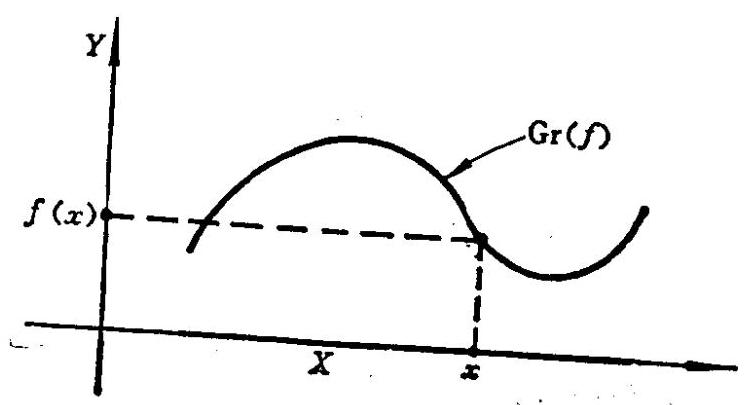
\includegraphics[max width=0.6\textwidth]{images/bo_d25ksc77aajc738obdgg_34_398_642_746_405_0.jpg}
\end{center}
\hspace*{3em} 

图 1-2

对于任一映射 $f : X \rightarrow  Y$ ,设 $A \subset  X$ 是一非空集合. 显然关系
$$g = \{ \left( {x,y}\right)  \mid  x \in  A,{xfy}\}$$

是从 $A$ 到 $Y$ 的一个映射.

定义 映射 $g : A \rightarrow  Y$ 称为映射 $f : X \rightarrow  Y$ 在 $A$ 上的限制,记为 ${\left. f\right| }_{A}$ . 如果一个映射 $h : A \rightarrow  Y$ 是映射 $f : X \rightarrow  Y$ 在 $A\left( { \subset  X}\right)$ 上的限制, 则我们称 $f$ 为 $h$ 的扩张.

例如考虑如下两个映射:
$$g = \left\{  {\left( {x,{x}^{2}}\right)  \mid  x \in  {\mathbf{R}}^{ + }}\right\}  ,f = \left\{  {\left( {x,{x}^{2}}\right)  \mid  x \in  \mathbf{R}}\right\}  ,$$

则 $g$ 是 $f$ 在 ${\mathbf{R}}^{ + }$ 上的限制,而 $f$ 是 $g$ 的扩张.

\section*{2. 单射、满射与一一映射}

首先我们介绍映射的象集与逆象集概念.

\footnote{
	
	① 《代数》(上册)(高级中学课本),人民教育出版社,1990年10月第 1 版。
	
	② $\mathrm{{Gr}}$ 是英文单词graph(图形)的头两个字母.
	
}

定义 设 $f : X \rightarrow  Y$ 是任一映射. $A \subset  X,B \subset  Y$ 是任意两个集合.

1) $f\left( A\right) \overset{\bigtriangleup }{ = }\{ y \in  Y \mid  \exists x \in  A$ 使 $y = f\left( x\right) \}$ 称为 $A$ 在 $f$ 下的象集.

2) ${f}^{-1}\left( B\right) \overset{ \bigtriangleup  }{ = }\{ x \in  X \mid  f\left( x\right)  \in  B\}$ 称为 $B$ 关于 $f$ 的逆象集.

显然,当 $A = X,B = Y$ 时, $f\left( X\right)  = \operatorname{Ran}\left( f\right) ,{f}^{-1}\left( Y\right)  =$  $\operatorname{Dom}\left( f\right)  = X$ .

可能出现这种情形:
$$A \subsetneq  X,f\left( A\right)  = \operatorname{Ran}\left( f\right) ,B \subsetneq  Y,{f}^{-1}\left( B\right)  = \varnothing ,$$

并且一般我们只能有下述包含关系式成立:
$$A \subset  {f}^{-1}\left( {f\left( A\right) }\right) ,f\left( {{f}^{-1}\left( B\right) }\right)  \subset  B.$$

例如,对上面所考虑过的映射 $f = \left\{  {\left( {x,{x}^{2}}\right)  \mid  x \in  \mathbf{R}}\right\}$ ,若取 $A = {\mathbf{R}}^{ + },B = {\mathbf{R}}_{ * }^{ - }$ ,则
$$f\left( {\mathbf{R}}^{ + }\right)  = \mathbf{R}\text{ an }\left( f\right)  = {\mathbf{R}}^{ + },{f}^{-1}\left( {\mathbf{R}}_{ * }^{ - }\right)  = \varnothing \text{ , }$$

${\mathbf{R}}^{ + } \subset  {f}^{-1}\left( {f\left( {\mathbf{R}}^{ + }\right) }\right)  = \mathbf{R}.$

\begin{center}
	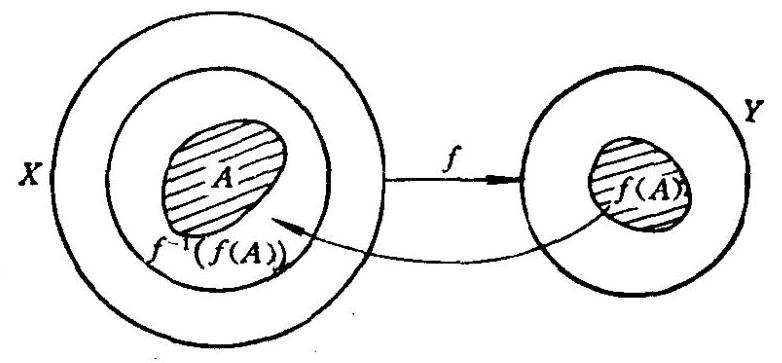
\includegraphics[max width=0.6\textwidth]{images/bo_d25ksc77aajc738obdgg_35_332_1285_782_363_0.jpg}
\end{center}
\hspace*{3em} 

\begin{center}
	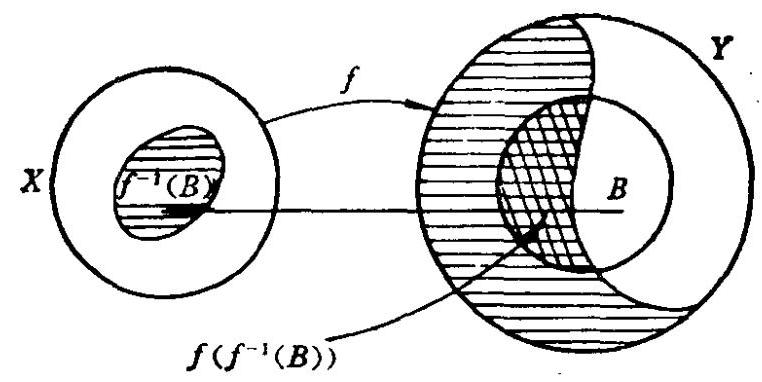
\includegraphics[max width=0.6\textwidth]{images/bo_d25ksc77aajc738obdgg_35_383_1664_762_382_0.jpg}
\end{center}
\hspace*{3em} 

图 1-3

关于映射 $f : X \rightarrow  Y$ 的值域 $f\left( X\right)  \subset  Y$ ,有下列三种情形值得我们特别考虑:

1) $f\left( X\right)  \subsetneq  Y$ ;

2) $f\left( X\right)  = Y$ ;

3) $\forall y \in  f\left( X\right) ,{f}^{-1}\left( y\right) \overset{\bigtriangleup }{ = }{f}^{-1}\left( {\{ y\} }\right)$ 是单点集.

与这三种情形对应的映射分类是:

定义 对映射 $f : X \rightarrow  Y$ ,

1) 若 $f\left( X\right)  \subsetneq  Y$ ,则称 $f$ 是内射;

2) 若 $f\left( X\right)  = Y$ ,则称 $f$ 是满射或全射;

3) 若 $\forall y \in  f\left( X\right) ,{f}^{-1}\left( y\right)$ 是单点集,则称 $f$ 是单射,

4)若 $f$ 既是单射,又是满射,则称 $f$ 是一一映射或满单射. 从单射的定义容易验证下 三个结论互相等价:

1) $f : X \rightarrow  Y$ 是单射;

2) 若 ${x}_{1},{x}_{2} \in  X$ 且 ${x}_{1} \neq  {x}_{2}$ ,则 $f\left( {x}_{1}\right)  \neq  f\left( {x}_{2}\right)$ ;

3) 若 ${x}_{1},{x}_{2} \in  X$ 且 $f\left( {x}_{1}\right)  = f\left( {x}_{2}\right)$ ,则 ${x}_{1} = {x}_{2}$ .

例 2 对任一映射 $f : X \rightarrow  Y$ ,映射 $f : X \rightarrow  f\left( X\right)$ 是满射.

例 3 对任一非空集合 $X$ ,映射 $x \mapsto  x,x \in  X$ 是一一映射, 称为从 $X$ 到 $X$ 上的恒等映射,记为 $i{d}_{X} : X \rightarrow  X$ .

例 4 前面考虑过的映射
$$f = \left\{  {\left( {x,{x}^{2}}\right)  \mid  x \in  \mathbf{R}}\right\}$$

不是单射,因为 $f\left( x\right)  = f\left( {-x}\right)  = {x}^{2},\forall x \in  \mathbf{R}$ ,但是 $f$ 在 ${\mathbf{R}}^{ + }$ 上的限制 ${\left. f\right| }_{{\mathrm{R}}^{ + }}$ 是从 ${\mathrm{R}}^{ + }$ 到 ${\mathrm{R}}^{ + }$ 上的一一映射.

对于两个映射, 如何判断它们是同一映射, 下面的命题给出了两个映射相等的充分必要条件.

命题 设 $f,g$ 是任意两个映射,则
$$f = g \Leftrightarrow  \operatorname{Dom}\left( f\right)  = \operatorname{Dom}\left( g\right) ,\;\forall x \in  \operatorname{Dom}\left( f\right) ,f\left( x\right)  =$$

$g\left( x\right)$ .

证明 首先由映射的定义, 我们有

$f = \{ \left( {x,y}\right)  \mid  {xfy}\} ,\operatorname{Dom}\left( f\right)  = \{ x \mid$ 存在唯一的 $y,{xfy}\} ,$

$\mathbf{g} = \{ \left( {x,y}\right)  \mid  {xyy}\} ,\operatorname{Dom}\left( g\right)  = \{ x \mid$ 存在唯一的 $y,{xyy}\} .$

现在设 $f = g$ . 那末 $\forall x \in  \operatorname{Dom}\left( f\right)$ ,存在唯一的 $y$ 使得 ${xfy}$ 或 $y = f\left( x\right)$ ,从而 $\left( {x,y}\right)  \in  f$ ,故 $\left( {x,y}\right)  \in  g$ ,因此 $x \in  \operatorname{Dom}\left( g\right)$ , $y = g\left( x\right)$ 或
$$\operatorname{Dom}\left( f\right)  \subset  \operatorname{Dom}\left( g\right) ,\;\forall x \in  \operatorname{Dom}\left( f\right) ,f\left( x\right)  = g\left( x\right) .$$

由对称性, 同理可证
$$\operatorname{Dom}\left( g\right)  \subset  \operatorname{Dom}\left( f\right) ,\;\forall x \in  \operatorname{Dom}\left( g\right) ,g\left( x\right)  = f\left( x\right) .$$

此即表明
$$\operatorname{Dom}\left( f\right)  = \operatorname{Dom}\left( g\right) ,\;\forall x \in  \operatorname{Dom}\left( f\right) ,f\left( x\right)  = g\left( x\right) .$$

反之,设 $\operatorname{Dom}\left( f\right)  = \operatorname{Dom}\left( g\right) ,\forall x \in  \operatorname{Dom}\left( f\right) ,f\left( x\right)  =$  $g\left( x\right)$ . 那末 $\forall \left( {x,y}\right)  \in  f,x \in  \operatorname{Dom}\left( f\right) ,y = f\left( x\right)$ ,从而 $x \in$  $\operatorname{Dom}\left( g\right) ,y = g\left( x\right)$ ,故 $\left( {x,y}\right)  \in  g$ ,因此 $f \subset  g$ .

同理可证 $g \subset  f$ . 因此 $f = g$ . 命题证毕.

下面我们介绍用逆关系与复合关系定义的逆映射 与复合映射.

\section*{3. 逆映射与复合映射}

定义 设 $f : X \rightarrow  Y$ 是任一映射. 如果 $f\left( X\right)  = Y$ 并且 $f$ 的逆关系 ${f}^{-1} = \{ \left( {y,x}\right)  \mid  {xfy}\}$ 也是一个映射,则我们称 $f$ 是可逆的, ${f}^{-1}$ 称为 $f$ 的逆映射.

由上述定义可知,若映射 $f : X \rightarrow  Y$ 可逆,则

1) ${f}^{-1}$ 是从 $Y$ 到 $X$ 上的映射,因为 $\operatorname{Dom}\left( {f}^{-1}\right)  = \operatorname{Ran}\left( f\right)  =$  $Y$ .

2) ${f}^{-1} : Y \rightarrow  X$ 也是可逆的,并且 ${\left( {f}^{-1}\right) }^{-1} = f$ .

例 5 考虑 $f = \{ \left( {x,x + 1}\right)  \mid  x \in  \mathbf{R}\}$ .

显然 $f$ 是从 $\mathbf{R}$ 到 $\mathbf{R}$ 上的映射,并且由于
\begin{align*}
	&{f}^{-1} = \{ \left( {y,x}\right)  \mid  {xfy}\}\\
	&= \{ \left( {y,x}\right)  \mid  x \in  \mathbf{R},y = x + 1\}\\
	&= \{ \left( {y,y - 1}\right)  \mid  y \in  \mathbf{R}\} \text{ , }
\end{align*}

及 $\forall y \in  3,y{f}^{-1}{x}_{1},y{f}^{-1}{x}_{2} \Rightarrow  {x}_{1} = y - 1,{x}_{2} = y - 1 \Rightarrow  {x}_{1} =$  ${x}_{2}$ ,故 ${f}^{-1}$ 也是一个映射,因此 $f$ 是可逆的.

例 6 考虑 $f = \left\{  {\left( {x,{x}^{2} + 1}\right)  \mid  x \in  \mathbf{R}}\right\}$ .

容易验证 $f$ 是从 $\mathbf{R}$ 到 $Y = \operatorname{Ran}\left( f\right)  = \left\{  {y \in  \mathbf{R} \mid  y = {x}^{2} + 1}\right.$ . $x \in$  $\mathbf{R}\}  = \{ y \in  \mathbf{R} \mid  y - 1 \geq  0\}  = \{ y \in  \mathbf{R} \mid  y \geq  1\}$ 上的映射.

由于
\begin{align*}
	&{f}^{-1} = \{ \left( {y,x}\right)  \mid  {xfy}\}\\
	&= \left\{  {\left( {y,x}\right)  \mid  x \in  \mathbf{R},y = {x}^{2} + 1}\right\}\\
	&= \{ \left( {y, \pm  \sqrt{y - 1}}\right)  \mid  y \geq  1\}
\end{align*}

及 $\forall y > 1,y{f}^{-1}\left( \sqrt{y - 1}\right) ,y{f}^{-1}\left( {-\sqrt{y - 1}}\right)$ ,但 $\sqrt{y - 1} \neq$  $- \sqrt{y - 1}$ ,故 ${f}^{-1}$ 不是一个映射,从而 $f$ 不可逆.

关于映射的复合, 我们首先证明下述定理.

定理 $1 \cdot  3 \cdot  1$ 设 $f,g$ 是任意两个映射,则

1) $g \circ  f$ 也是一个映射;

2) $g \circ  f$ 在 $x$ 处有定义当且仅当 $f$ 在 $x$ 处有定义, $g$ 在 $f\left( x\right)$ 处有定义, 于是
$$\operatorname{Dom}\left( {g \circ  f}\right)  = \operatorname{Dom}\left( f\right)  \cap  {f}^{-1}\left( {\operatorname{Dom}\left( g\right) }\right) ;$$

3) $\forall x \in  \operatorname{Dom}\left( {g \circ  f}\right) ,g \circ  f\left( x\right)  = g\left( {f\left( x\right) }\right)$ .

证明 1 )我们只需证明
$$\forall x,x\left( {g \circ  f}\right) {z}_{1},x\left( {g \circ  f}\right) {z}_{2} \Rightarrow  {z}_{1} = {z}_{2}.$$

根据复合关系的定义, $\exists {y}_{1},{y}_{2}$ 使得
$${xf}{y}_{1},{y}_{1}g{z}_{1};{xf}{y}_{2},{y}_{2}g{z}_{2}.$$

因为 $f$ 是映射,故 ${y}_{1} = {y}_{2}$ ,又因为 $g$ 是映射,故由 ${y}_{1}g{z}_{1},{y}_{1}g{z}_{2}$ 推得 ${z}_{1} = {z}_{2}$ .

2) $x \in  \operatorname{Dom}\left( {g \circ  f}\right)  \Leftrightarrow  \exists z$ 使 $x\left( {g \circ  f}\right) z$
\begin{align*}
	&\Leftrightarrow  \exists y\text{ 和 }z\text{ 使 }{xfy},{ygz}\\
	&\Leftrightarrow  x \in  \operatorname{Dom}\left( \dot{f}\right) ,y = \dot{f}\left( x\right)  \in  \operatorname{Dom}\left( g\right)\\
	&\Leftrightarrow  x \in  \operatorname{Dom}\left( f\right)  \cap  {f}^{-1}\left( {\operatorname{Dom}\left( g\right) }\right) .
\end{align*}

3) 由 2) 的证明推出.

根据此定理, 我们可以引进下述定义.

定义 设 $f,g$ 是任意两个映射,则 $g \circ  f$ 称为 $f$ 与 $g$ 的复合映射.

从图 1-4 可以理解 $g \circ  f$ 的意义.

\begin{center}
	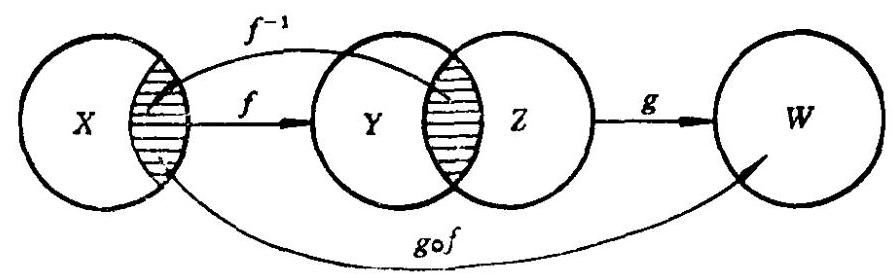
\includegraphics[max width=0.7\textwidth]{images/bo_d25ksc77aajc738obdgg_39_339_847_896_278_0.jpg}
\end{center}
\hspace*{3em} 

图 1-4

例7 设 $f = \left\{  {\left( {x,{x}^{2} + 1}\right)  \mid  x \in  \mathrm{R}}\right\}  ,g = \left\{  {\left( {y,\sqrt{y}}\right)  \mid  y \in  {\mathrm{R}}^{ + }}\right\}$ . 则
$$\operatorname{Dom}\left( {g \circ  f}\right)  = \operatorname{Dom}\left( f\right)  \cap  {f}^{-1}\left( {\operatorname{Dom}\left( g\right) }\right)  = \mathbf{R} \cap  {f}^{-1}\left( {\mathbf{R}}^{ + }\right)  =$$

$\mathbf{R} \cap  \mathbf{R} = \mathbf{R}$
$$\operatorname{Dom}\left( {f \circ  g}\right)  = \operatorname{Dom}\left( g\right)  \cap  {g}^{-1}\left( {\operatorname{Dom}\left( f\right) }\right)  = {\mathbf{R}}^{ + } \cap  {g}^{-1}\left( \mathbf{R}\right)  =$$

${\mathbf{R}}^{ + } \cap  {\mathbf{R}}^{ + } = {\mathbf{R}}^{ + }$
\begin{align*}
	&g \circ  f = \{ \left( {x,z}\right)  \mid  x \in  \mathbb{R}\text{ 并且存在 }y\text{ 使得 }{xfy},{ygz}\}\\
	&= \left\{  {\left( {x,z}\right)  \mid  x \in  \mathbf{R},y = {x}^{2} + 1,z = \sqrt{y}}\right\}\\
	&= \{ \left( {x,\sqrt{{x}^{2} + 1}}\right)  \mid  x \in  \mathbf{R}\} \text{ ; }
\end{align*}

$f \circ  g = \left\{  {\left( {x,z}\right)  \mid  x \in  {\mathbf{R}}^{ + }\text{ ,并且存在 }y\text{ 使得 }{xgy},{yfz}}\right\}$
\begin{align*}
	&= \left\{  {\left( {x,z}\right)  \mid  x \in  {\mathbf{R}}^{ + },y = \sqrt{x},z = {y}^{2} + 1}\right\}\\
	&= \left\{  {\left( {x,x + 1}\right)  \mid  x \in  {\mathbf{R}}^{ + }}\right\}  .
\end{align*}

利用映射的复合可以判断映射的单射性与满射性, 即成立下面的定理,

定理 $1 \cdot  3 \cdot  2$ 设 $f : X \rightarrow  Y$ 与 $g : Y \rightarrow  X$ 是任意两个映射,

1) 若 $g \circ  f = i{d}_{X}$ ,则 $f$ 是单射, $g$ 是满射;

2) 若 $g \circ  f = i{d}_{X},f \circ  g = i{d}_{Y}$ ,则 $f$ 与 $g$ 是一一映射,并且 ${f}^{-1} = g,{g}^{-1} = f.$

证明 1 )设 ${x}_{1},{x}_{2} \in  X$ 使得 $f\left( {x}_{1}\right)  = f\left( {x}_{2}\right)$ . 那末
\begin{align*}
	&{x}_{1} = i{d}_{X}\left( {x}_{1}\right)  = g \circ  f\left( {x}_{1}\right)  = g\left( {f\left( {x}_{1}\right) }\right)\\
	&= g\left( {f\left( {x}_{2}\right) }\right)  = g \circ  f\left( {x}_{2}\right)  = i{d}_{X}\left( {x}_{2}\right)  = {x}_{2},
\end{align*}

因此 $f$ 是单射.

为了证明 $g$ 是满射,设 $x \in  X$ ,令 $y = f\left( x\right)$ . 则
$$x = i{d}_{X}\left( x\right)  = g \circ  f\left( x\right)  = g\left( {f\left( x\right) }\right)  = g\left( y\right) ,$$

因此 $g$ 是满射.

2 ,若 $g \circ  f = i{d}_{X},f \circ  g = i{d}_{Y}$ ,则由 1 )知 $f,g$ 都是一一映射,为了证明 ${f}^{-1} = g,{g}^{-1} = f$ ,我们只需证明
$${f}^{-1}\left( y\right)  = g\left( y\right) ,y \in  Y,{g}^{-1}\left( x\right)  = f\left( x\right) ,x \in  X.$$

事实上,由于 ${f}^{-1} \circ  f = i{d}_{X},{g}^{-1} \circ  g = i{d}_{Y}$ ,故
\begin{align*}
	&g\left( y\right)  = \left( {{f}^{-1} \circ  f}\right) \left( {g\left( y\right) }\right)  = {f}^{-1}\left( {f\left( {g\left( y\right) }\right) }\right)  = {f}^{-1}\left( y\right) ,y \in  Y,\\
	&f\left( x\right)  = \left( {{g}^{-1} \circ  g}\right) \left( {f\left( x\right) }\right)  = {g}^{-1}\left( {g\left( {f\left( x\right) }\right) }\right)  = {g}^{-1}\left( x\right) ,x \in  X.
\end{align*}

最后作为映射的一个应用, 我们来介绍集合的可数性.

\section*{4. 集合的可数性}

定义 设 $X$ 是任一集合.

1) 我们称 $X$ 是有限集,如果 $X$ 是空集,或者存在 $n \in  \mathbf{N}$ 及一个一一映射 $f : \{ 1,2,\cdots ,n\}  \rightarrow  X$ . 在第一种情形下称 $X$ 有 0 个元素,在第二种情形下称 $X$ 有 $n$ 个元素.

2) 我们称 $X$ 是无限集,如果它不是有限集.

3) 我们称 $X$ 是可数无限集,如果存在一一映射 $f : \mathbf{N} \rightarrow  X$ .

4) 我们称 $X$ 是可数集,如果 $X$ 是有限集或可数无限集.

5) 我们称 $X$ 是不可数集,如果 $X$ 不是可数集.

例 8 对每一个 $n \in  \mathbf{N}$ ,集合 $\{ 1,2,\cdots ,n\}$ 是有 $n$ 个元素的有限集,而集合 $\mathbf{N}$ 是可数无限集.

例 9 整数集 $\mathbf{Z}$ 是可数无限集. 因为我们有一一映射 $f : \mathbf{N} \rightarrow$  ${Z}_{3}$
$$f\left( n\right)  = \left\{  \begin{array}{ll} k, & \text{ 若 }n = {2k} + 1\;\left( {k = 0,1,2}\right) \\   - k, & \text{ 若 }n = {2k}\;\left( {k = 1,2,\cdots }\right) . \end{array}\right.$$

定理 $1 \cdot  3 \cdot  3$ 设 $X$ 是任一非空集合. $X$ 是可数集的充分必要条件是存在一个满射 $f : \mathbf{N} \rightarrow  X$ .

证明 必要性 设 $X$ 是可数集. 如果 $X$ 是无限集,则由定义, 存在一一映射 $f : \mathbf{N} \rightarrow  X$ ; 如果 $X$ 是有 $n$ 个元素的有限集,则存在一一映射 $g : \{ 1,2,\cdots ,n\}  \rightarrow  X$ . 现在定义映射 $f : \mathbf{N} \rightarrow  X$ 为:
$$f\left( m\right)  = \left\{  \begin{array}{l} g\left( m\right) m = 1,2,\cdots ,n; \\  g\left( 1\right) m = n + 1,n + 2,\cdots \cdots  \end{array}\right.$$

显然 $f$ 是满射.

充分性 设存在满射 $f : \mathbf{N} \rightarrow  X$ . 如果 $X$ 是有限集,则充分性成立. 因此不妨设 $X$ 是无限集.

在 $\mathbf{N}$ 上定义关系 $\mathcal{R}$ 如下:
$$n,m \in  \mathbf{N},n\mathcal{B}m \Leftrightarrow  f\left( n\right)  = f\left( m\right) .$$

容易验证 $\mathcal{R}$ 是 $\mathbf{N}$ 上的一个等价关系.

下面我们定义两个映射 $h : \mathbf{N} \rightarrow  \mathbf{N}/\mathcal{B}$ 与 $g : \mathbf{N}/\mathcal{B} \rightarrow  X$ .

首先定义映射 $g : \mathbf{N}/\mathcal{R} \rightarrow  X$ 如下:
$$g\left( \widetilde{n}\right)  = f\left( n\right) ,\;\forall \widetilde{n} \in  \mathbf{N}/\mathcal{R}.$$

显然 $g$ 是单射.

其次我们归纳地定义映射 $h : \mathbf{N} \rightarrow  \mathbf{N}/\mathcal{R}$ .

$h\left( 1\right)  = \overset{⏜}{{k}_{1}} = \overset{⏜}{1}$

$h\left( 2\right)  = \widetilde{{k}_{2}}$ . 这里 ${k}_{2}$ 是不属于 $\widetilde{1}$ 的最小自然数.

现在假设 $h\left( 1\right)  = \widetilde{{k}_{1}},h\left( 2\right)  = \widetilde{{k}_{2}},\cdots ,h\left( m\right)  = \widetilde{{k}_{m}}$ 已经定义好了, 我们令

$h\left( {m + 1}\right)  = {\widetilde{k}}_{m + 1}$ ,这里 ${k}_{m + 1}$ 是不属于 ${\widetilde{k}}_{1},{\widetilde{k}}_{2},\cdots ,{\widetilde{k}}_{m}$ 的最小自然数.

由于 $X$ 是无限集, $g$ 是单射,故 $\mathbf{N}/\mathcal{R}$ 也是无限集,因此上述定义 $h$ 的过程可以无限地继续下去. 从而映射 $h : \mathbf{N} \rightarrow  \mathbf{N}/\mathcal{R}$ 就完全归纳地定义了.

现在我们来证明复合映射 $g \circ  h : \mathbf{N} \rightarrow  X$ 是一一映射,从而 $X$ 是可数无限集.

首先证明 $g \circ  h$ 是单射. 为此设 $n,m \in  \mathbf{N}$ 且 $n \neq  m$ . 那末
$$g \circ  h\left( n\right)  = g\left( \widetilde{{k}_{n}}\right) ,\;g \circ  h\left( m\right)  = g\left( \widetilde{{k}_{m}}\right) .$$

由于 $\widetilde{{k}_{n}} = \widetilde{{k}_{m}},g$ 是单射,所以 $g \circ  h\left( n\right)  \neq  g \circ  h\left( m\right)$ .

为了证明 $g \circ  h$ 是满射,设 $a \in  X$ . 由于 $f$ 是满射,故存在 $n \in  \mathbf{N}$ 使得 $f\left( n\right)  = a$ . 令 ${k}_{m}$ 是 $\widetilde{n}$ 中最小自然数,那末 $g \circ  h\left( m\right)  = g\left( \widetilde{{k}_{m}}\right)  =$  $f\left( {k}_{m}\right)  = f\left( n\right)  = a.$

推论 1 若 $X$ 是可数集, $Y \subset  X$ 是任一子集,则 $Y$ 也是可数集.

证明 如果 $Y$ 是空集,则推论成立. 因此不妨设 $Y \neq  \varnothing$ . 令 ${x}_{0} \in  Y$ . 由于 $X$ 可数,故存在满射 $g : \mathbf{N} \rightarrow  X$ . 现在定义映射 $f : \mathbf{N} \rightarrow$  $Y$ 为:
$$f\left( n\right)  = \left\{  \begin{array}{ll} g\left( n\right. & \text{ 若 }g\left( n\right)  \in  Y; \\  {x}_{0} & \text{ 若 }g\left( n\right)  \in  Y. \end{array}\right.$$

则 $f$ 是满射,因此 $Y$ 是可数集.

推论 2 若 ${X}_{1},{X}_{2},\cdots ,{X}_{n},\cdots \cdots$ 是可数多个可数集,则 $\mathop{\bigcup }\limits_{{k = 1}}^{n}{X}_{k},\mathop{\bigcup }\limits_{{k \in  \mathbb{N}}}{X}_{k}$ 也是可数集.

证明 由于对任意的 $n \in  \mathbf{N},\mathop{\bigcup }\limits_{{k = 1}}^{n}{X}_{k} \subset  \mathop{\bigcup }\limits_{{k \in  \mathbf{N}}}{X}_{k}$ ,根据推论1, 我们只需证明 $\mathop{\bigcup }\limits_{{k \in  \mathrm{N}}}{X}_{k}$ 是可数集.

不妨设每一个 ${X}_{k} \neq  \varnothing$ ,否则可以把那些空集删去. 由于 ${X}_{k}$ 是可数集,故存在满射 ${f}_{k} : \mathbf{N} \rightarrow  {X}_{k}$ . 下面我们定 义映射 $f : \mathbf{N} \rightarrow$  $\mathop{\bigcup }\limits_{{k \in  \mathrm{N}}}{X}_{k}$ 如下:

首先,对每一个 $n \in  \mathbf{N}$ 可唯一的分解成
$$n = {2}^{k - 1}\left( {{2m} - 1}\right) \;\left( {k,m \in  \mathbf{N}}\right)$$

的形式. 我们令 $f\left( n\right)  = {f}_{k}\left( m\right)$ ,则 $f$ 是满射. 事实上,设 $x \in$  $\mathop{\bigcup }\limits_{{k \in  N}}{X}_{k}$ . 于是存在 $k \in  \mathbf{N}$ 使得 $x \in  {X}_{k}$ ,从而存在 $m \in  \mathbf{N}$ 使得 $x =$  ${f}_{k}\left( m\right)$ . 若令 $n = {2}^{k - 1}\left( {{2m} - 1}\right)$ ,则 $f\left( n\right)  = f\left( {{2}^{k - 1}\left( {{2m} - 1}\right) }\right)  =$  ${f}_{k}\left( m\right)  = x$ ,因此 $f$ 是满射. 故 $\mathop{\bigcup }\limits_{{k \in  \mathrm{N}}}{X}_{k}$ 是可数集.

例 10 有理数集 $\mathbf{Q}$ 是可数集.

事实上,对每一个 $n \in  \mathbf{N}$ ,令
$${\mathbf{Q}}_{n} = \left\{  {\left. \frac{m}{n}\right| \;m \in  \mathbf{Z},\text{ 且 } - {n}^{2} \leq  m \leq  {n}^{2}}\right\}  ,$$

则 ${\mathbf{Q}}_{n}$ 是有限集,并且 $\mathbf{Q} = \mathop{\bigcup }\limits_{{n \in  \mathbf{N}}}{\mathbf{Q}}_{n}$ ,因此由推论 2 知 $\mathbf{Q}$ 是可数集.

推论 3 若 ${X}_{1},{X}_{2},\cdots ,{X}_{n}$ 是可数集,则乘积 ${X}_{1} \times  {X}_{2} \times  \cdots$  $\times  {X}_{n}$ 也是可数集.

证明 不妨设每一个 ${X}_{k} \neq  \varnothing$ ,否则 ${X}_{1} \times  {X}_{2} \times  \cdots  \times  {X}_{n} = \varnothing$ , 它显然是可数集.

首先由分解式 $n = {2}^{k - 1}\left( {{2m} - 1}\right)$ 及映射 $h : \mathbf{N} \rightarrow  \mathbf{N} \times  \mathbf{N},h\left( n\right)  =$  $\left( {k,m}\right) \;\left( {n \in  \mathbf{N}}\right)$ 知 $h$ 是一一映射,因此 $\mathbf{N} \times  \mathbf{N}$ 是可数集.

设 $A\text{ 、 }B$ 是两个可数集,于是存在满射
$${f}_{1} : N \rightarrow  A,{f}_{2} : N \rightarrow  B.$$

定义映射 $g : \mathbf{N} \times  \mathbf{N} \rightarrow  A \times  B$ 为:
$$g\left( {n,m}\right)  = \left( {{f}_{1}\left( n\right) ,{f}_{2}\left( m\right) }\right) \;\left( {n,m}\right)  \in  \mathbf{N} \times  \mathbf{N},$$

则 $g$ 是满射. 因此 $g \circ  h : \mathbf{N} \rightarrow  A \times  B$ 也是满射,从而 $A \times  B$ 是可数集.

现在假设 ${X}_{1} \times  {X}_{2} \times  \cdots  \times  {X}_{n - 1}$ 是可数集,那末 $\left( {{X}_{1} \times  {X}_{2} \times  \cdots }\right.$  $\left. {\times {X}_{n - 1}}\right)  \times  {X}_{n}$ 是可数集. 从而存在满射
$$f : \mathrm{N} \rightarrow  \left( {{X}_{1} \times  {X}_{2} \times  \cdots  \times  {X}_{n - 1}}\right)  \times  {X}_{n}.$$

另一方面, 若定义映射
$$g : \left( {{X}_{1} \times  {X}_{2} \times  \cdots  \times  {X}_{n - 1}}\right)  \times  {X}_{n} \rightarrow  {X}_{1} \times  {X}_{2} \times  \cdots  \times  {X}_{n - 1} \times  {X}_{n}$$

为
$$g\left( {\left( {{x}_{1},{x}_{2},\cdots ,{x}_{n - 1}}\right) ,{x}_{n}}\right)  = \left( {{x}_{1},{x}_{2},\cdots ,{x}_{n - 1},{x}_{n}}\right) ,$$

则 $g$ 是一一映射,从而 $g \circ  f : \mathbf{N} \rightarrow  {X}_{1} \times  {X}_{2} \times  \cdots  \times  {X}_{n}$ 是满射,因此 ${X}_{1} \times  {X}_{2} \times  \cdots  \times  {X}_{n}$ 是可数集.

不可数集的一个简单例子就是下面的例.

例11 N的幂集 ${2}^{\mathrm{N}}$ 是不可数集。

为此我们只需证明不存在任何满射 $f : \mathbf{N} \rightarrow  {2}^{\mathbf{N}}$ . 设 $f : \mathbf{N} \rightarrow  {2}^{\mathbf{N}}$ 是任一映射. 对每一个 $n \in  \mathbf{N},f\left( n\right)$ 是 $\mathbf{N}$ 的一个子集。那末我们有
$$n \in  f\left( n\right) \text{ 或 }n \in  f\left( n\right) .$$

构造 $\mathbf{N}$ 的一个子集 $E$ 如下:
$$E = \{ n \in  \mathbf{N} \mid  n \in  f\left( n\right) \} ,$$

显然 $E \in  {2}^{\mathbb{N}}$ .

下面证明 $E \in  f\left( \mathbf{N}\right)$ . 用反证法,假设存在 ${n}_{0} \in  \mathbf{N}$ ,使得 $F\left( {n}_{0}\right)  = E$ 。那末由 $E$ 的定义知

若 ${n}_{0} \in  E$ ,则 ${n}_{0} \in  f\left( {n}_{0}\right)  = E$ ;

若 ${n}_{0} \in  E$ ,则 ${n}_{0} \in  f\left( {n}_{0}\right)  = E$ ,

这显然是矛盾的. 因此 $f$ 不是满射. 故由定理 $1 \cdot  3 \cdot  3$ 知 ${2}^{N}$ 是不可数集.

\section*{习 题}

1. 指出下列关系中哪些是函数关系:

1) ${f}_{1} = \{ \left( {x,y}\right)  \mid  x \in  \mathbf{R},y \in  \mathbf{N}\}$ ;

2) ${f}_{2} = \{ \left( {x,y}\right)  \mid  0 \leq  x \leq  1,0 \leq  y \leq  1\}$ ;

3) ${f}_{3} = \left\{  {\left( {x,y}\right)  \mid  x \in  R-\{ 0\} ,y = \frac{1}{{x}^{2}}}\right\}$ ;

4) ${f}_{4} = \{ \left( {x,y}\right)  \mid  x \in  \mathbf{R},y = \left| x\right| \}$ .

2. 设 $f = \left\{  {\left( {x,{x}^{2} - 1}\right)  \mid  x \in  \mathrm{R}}\right\}  ,g = \left\{  {\left( {y,\sqrt{y}}\right)  \mid  y \in  {\mathrm{R}}^{ + }}\right\}$ 分别写出 $\operatorname{Dom}\left( {g \circ  f}\right) ,\operatorname{Dom}\left( {f \circ  g}\right) ,g \circ  f$ 及 $f \circ  g$ .

3. 设映射 ${f}_{1},{f}_{2},{f}_{3}$ ,定义如下:
\begin{align*}
	&{f}_{1} = \{ \left( {x,y}\right)  \mid  x \in  R,y = x + 1\} ,\\
	&{f}_{2} = \left\{  {\left( {x,y}\right)  \mid  x \in  {R}^{ + },y = \sqrt{x}}\right\}  ,\\
	&{f}_{3} = \{ \left( {x,y}\right)  \mid  x \in  \mathrm{R},y = \sqrt[3]{x}\} ,
\end{align*}

试确定下列各映射, 并且写出各自的定义域.
$${f}_{2} \circ  {f}_{1},{f}_{1} \circ  {f}_{2},{f}_{1} \circ  {f}_{3},{f}_{3} \circ  {f}_{1},{f}_{2} \circ  {f}_{3},{f}_{8} \circ  {f}_{2}.$$

4. 设 $f : X \rightarrow  Y$ 是任一映射.

1) 设 $A,B \subset  X$ 是任意两个集合,证明:
\begin{align*}
	&f\left( {A \cup  B}\right)  = f\left( A\right)  \cup  f\left( B\right) ,\\
	&f\left( {A \cap  B}\right)  \subset  f\left( A\right)  \cap  f\left( B\right) ,\\
	&f\left( {A - B}\right)  \supset  f\left( A\right)  - f\left( B\right) .
\end{align*}

若 $f$ 为单射,则 $f\left( {A \cap  B}\right)  = f\left( A\right)  \cap  f\left( B\right) ,f\left( {A - B}\right)  = f\left( A\right)  - f\left( B\right)$ .

2) 设 $C,D \subset  Y$ 是任意两个集合,证明:
\begin{align*}
	&{f}^{-1}\left( {C \cup  D}\right)  = {f}^{-1}\left( C\right)  \cup  {f}^{-1}\left( D\right) ,\\
	&{f}^{-1}\left( {C \cap  D}\right)  = {f}^{-1}\left( C\right)  \cap  {f}^{-1}\left( D\right) ,\\
	&{f}^{-1}\left( {C - D}\right)  = {f}^{-1}\left( C\right)  - {f}^{-1}\left( D\right) .
\end{align*}

5. 设 $f : X \rightarrow  Y$ 是任一映射. $A \subset  X,B \subset  Y$ ,证明:

1) $f\left( A\right)  = \varnothing  \Leftrightarrow  A = \varnothing$ :

2) ${f}^{-1}\left( B\right)  = \varnothing  \Leftrightarrow  B \cap  f\left( X\right)  = \varnothing$ : 若 $f$ 是满射,则 ${f}^{-1}\left( B\right)  = \varnothing  \Leftrightarrow$  $B = \varnothing$ :

3) ${\left( {\left. f\right| }_{A}\right) }^{-1}\left( B\right)  = A \cap  {f}^{-1}\left( B\right)$ ;

4) $A \subset  {f}^{-1}\left( {f\left( A\right) }\right) ,f\left( {{f}^{-1}\left( B\right) }\right)  \supset  B$ ;

5) $f$ 是单射 $\Leftrightarrow$ 对每一个 $A = X,{f}^{-1}\left( {f\left( A\right) }\right)  = A$ ,

6) $f$ 是满射 $\Leftrightarrow$ 对每一个 $B \subset  Y,f\left( {{f}^{-1}\left( B\right) }\right)  = B$ ;

7) $f$ 是一一映射 $\Leftrightarrow$ 对每一个 $A \subset  X,B \subset  Y,{f}^{-1}\left( {f\left( A\right) }\right)  = A$ , $f\left( {{f}^{-1}\left( B\right) }\right)  = B.$

6. 证明第 3 题中的每一个映射 ${f}_{1},{f}_{2},{f}_{3}$ 都是可逆的,并写出它们的逆映射 ${f}_{i}^{-1}\left( {i = 1,2,3}\right)$ . 证明:

$\operatorname{Dom}\left( {f}_{i}\right)  = \operatorname{Ran}\left( {f}_{i}^{-1}\right) ,\operatorname{Ran}\left( {f}_{i}\right)  = \operatorname{Dom}\left( {f}_{i}^{-1}\right) \left( {i = 1,2,3}\right) .$

7. 设 $f$ 是任一映射. 证明: 如果存在映射 $g$ 与 $h$ 使得 $g \circ  f = i{d}_{D \circ  m\left( f\right) }$ , $f \circ  h = i{d}_{\text{ Ran }\left( f\right) }$ ,则 $f$ 是可逆的,并且 ${f}^{-1} = h = g$ .

8. 证明: 若 $f$ 与 $g$ 是单射,则 $g \circ  f$ 也是单射,并且 ${\left( g \circ  f\right) }^{-1} = {f}^{-1} \circ  {g}^{-1}$ .

9. 设 $f,g : X \rightarrow  \mathrm{R}$ 是任意两个映射. 定义映射 $f + g,{fg} : X \rightarrow  \mathrm{R}$ 为:
$$\left( {f + g}\right) \left( x\right)  = f\left( x\right)  + g\left( x\right) ,\left( {fg}\right) \left( x\right)  = f\left( x\right)  \cdot  g\left( x\right) ,x \in  X$$

现在设 $E \subset  X$ 是任一集合. 映射 ${\chi }_{E} : X \rightarrow  \{ 0,1\}$ ,
$${\chi }_{E}\left( x\right)  = \left\{  \begin{array}{l} 1,\text{ 若 }x \in  E, \\  0,\text{ 若 }x \in  E. \end{array}\right.$$

称为 $E$ 的特征函数. 证明: 对任意的 $A,B \subset  X$ ,

1) ${\chi }_{A \cap  B} = {\chi }_{A} \cdot  {\chi }_{B}$ ; 2) ${\chi }_{A \cup  B} = {\chi }_{A} + {\chi }_{B} - {\chi }_{A \cap  B}$ ,

3) ${\chi }_{A - B} = {\chi }_{A}\left( {1 - {\chi }_{B}}\right)$ .

10. 设 $f : X \rightarrow  Y$ 是任一映射, $A \subset  X$ 是任一非空集合. 我们称 $A$ 关于 $f$ 不变,如果 $f\left( A\right)  = A$ . 定义 $X$ 的子集 $B$ 如下:

$B = \{ x \in  X \mid$ 存在 $X$ 的一列元素 ${x}_{1},{x}_{2}\cdots \cdots$ 使得
$$\left. {x = {x}_{1},{x}_{n} = f\left( {x}_{n + 1}\right) }\right\}  .$$

证明 $B$ 是 $X$ 的关于 $f$ 不变的最大子集合.

11. 设 $E$ 是 $\mathbf{N}$ 的所有有限集的集合,定义映射 $f : E \rightarrow  \mathbf{N}$ 如下:
$$f\left( A\right)  = \left\{  \begin{array}{l} 0,\text{ 若 }A = \varnothing , \\  \mathop{\sum }\limits_{{x \in  A}}x,\text{ 若 }A \neq  \varnothing . \end{array}\right.$$

1) 设 ${A}_{n} = \{ 1,2,\cdots ,n\}$ ,计算 $f\left( {A}_{n}\right)$ ;

2) 证明 $f$ 不是单射;

3) 证明 $f$ 是满射;

4) 计算集合 ${f}^{-1}\left( 4\right)$ 的元素的个数.

12. 证明: 任一可数集的所有有限子集所组成的集合是可数集.

13. 设 $A,B$ 是任意两个集合. 如果存在一一映射 $f : A \rightarrow  B$ ,则称 $A$ 与 $B$ 是等势的.

1) 证明: 对任一非空集合 $X,X$ 与 ${2}^{X}$ 不等势;

2) 证明:[0, 1[、]0, 1], [0, 1[, [0, 1], ]0, + ∞[, [0, + ∞[ 互相等势; (这些集合的定义可参见第 2 章 $§5$ .)

3) 证明: 若 ${S}^{2}$ 表示 ${R}^{3}$ 中的球面,则对每一个 $a \in  {S}^{2},{S}^{2} - \{ a\}$ 与 ${R}^{2}$ 等势.

14. 设 $\left( {X, \preccurlyeq  }\right)$ 是任一全序集, $f : X \rightarrow  X$ 是任一映射,它具有性质:

若 $x,y \in  X$ ,且 $x \prec  y$ ,则 $f\left( x\right)  \prec  f\left( y\right)$ .

证明: 1) $f$ 是单射;

2) 若 $f\left( x\right)  \prec  f\left( y\right)$ ,则 $x \prec  y$ .

15. 设 $X\text{ 、 }Y$ 是任意两个集合. 我们用 $E$ 表示所有定义域包含在 $X$ 中而值域包含在 $Y$ 中的映射的集合.

在 $E$ 上定义关系 $\mathcal{R}$ 如下:

$f,g \in  E,f\mathcal{R}g \Leftrightarrow  \operatorname{Dom}\left( f\right)  \subset  \operatorname{Dom}\left( g\right)$ 且 $g$ 是 $f$ 的扩张.

试问: 1) $\mathcal{B}$ 是 $E$ 上的偏序关系吗?

2) $\mathcal{B}$ 是 $E$ 上的序关系吗?

16. 设 ${X}_{1},{X}_{2}$ 是两个集合, ${\mathcal{R}}_{i}$ 是 ${X}_{i}$ 上的一个等价关系,定义投影映射 ${p}_{i} : {X}_{i} \rightarrow  {X}_{i}/{\mathcal{R}}_{i}\left( {i = 1,2}\right)$ 为:

$\forall x \in  {X}_{i},{p}_{i}\left( x\right)  = x,x$ 是 $x$ 关于 ${\mathcal{R}}_{i}$ 的等价类.

现在设映射 $f : {X}_{1} \rightarrow  {X}_{2}$ 满足下述性质
$${x}^{\prime },{x}^{\prime \prime } \in  {X}_{1},{x}^{\prime }{\mathcal{R}}_{1}{x}^{\prime \prime } \Rightarrow  f\left( {x}^{\prime }\right) {\mathcal{R}}_{2}f\left( {x}^{\prime \prime }\right) .$$

证明: 1) 存在映射 $F : {X}_{1}/{\mathcal{A}}_{1} \rightarrow  {X}_{2}/{\mathcal{A}}_{2}$ 使得下述图形可交换:

\begin{center}
	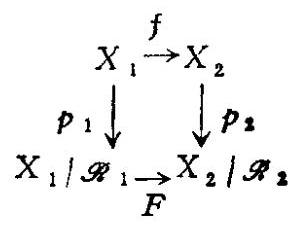
\includegraphics[max width=0.2\textwidth]{images/bo_d25ksc77aajc738obdgg_47_680_1538_295_225_0.jpg}
\end{center}
\hspace*{3em} 

即证明等式 $F{p}_{1} = {p}_{2}f$ 成立.

2) 如果 $f$ 是满射,则 $F$ 也是满射.